% -*- latex -*-
%
% The SAND document class is maintained at:
%
%    http://www.cs.sandia.gov/SANDreport/sandHome.html
%
% This page also as instructions and documentation on commands.
%
\documentclass[12pt,report]{SANDreport}

\SANDnum{SAND2013-xxxx}
\SANDprintDate{December 2013}

\title{A Pervasive Parallel Framework for Visualization: Final Report for
  FWP~10-014707}
\author{Kenneth~Moreland}
\SANDauthor{Kenneth~Moreland}
\date{} % Leave empty


\usepackage{amsfonts}
\usepackage{amssymb}
\usepackage{amsmath}
\usepackage{booktabs}
\usepackage{graphicx}
\usepackage{varioref}
\usepackage{fancyvrb}
\usepackage{ifthen}
\usepackage{cite}
\usepackage{subfig}
\usepackage{xspace}

\usepackage{lmodern}

\usepackage{makeidx}
\makeindex

\usepackage[pdfborder={0 0 0}]{hyperref}
\usepackage{verbatim}

\usepackage{color}
\definecolor{yellow}{rgb}{1,1,0}
\definecolor{black}{rgb}{0,0,0}
\definecolor{ltcyan}{rgb}{.75,1,1}
\definecolor{red}{rgb}{1,0,0}
\definecolor{gray}{rgb}{.6,.6,.6}
\definecolor{darkred}{rgb}{0.5,0,0}
\definecolor{darkgreen}{rgb}{0,0.5,0}

\definecolor{daxidentifier}{rgb}{0,0,1}
\definecolor{daxnamespace}{rgb}{0.5,0,0}
\definecolor{daxmacro}{rgb}{0.5,0,0}
\definecolor{daxsignature}{rgb}{0,0.5,0}

\usepackage{listings}
\lstloadlanguages{C,C++}
\lstset{fontadjust=false,basicstyle=\scriptsize\ttfamily}
%% \lstset{numbers=left, numberstyle=\tiny, stepnumber=1, numbersep=2pt}
\lstdefinelanguage{Dax}{
  morekeywords={struct,class,public,typedef, void, template, return, operator, const, for, int},
  morekeywords={[2]_1,_2,_3,_4, In, Out, Point, Field, Topology,
                   Id, Id3, Tuple, Vector2,Vector3,Vector4,
                   WorkletMapField, WorkletMapCell,
                   ParametricCoordinates, CellDerivative},
  morekeywords={[3]DAX_CONT_EXPORT,DAX_EXEC_EXPORT,DAX_EXEC_CONT_EXPORT},
  morekeywords={[4]dax,exec,cont,math},
  morekeywords={[5]ControlSignature, ExecutionSignature}
}
\lstset{language=Dax}
\lstset{
  keywordstyle=\bfseries,
  keywordstyle=[2]\color{daxidentifier},
  keywordstyle=[3]\color{daxmacro},
  keywordstyle=[4]\color{daxnamespace},
  keywordstyle=[5]\color{daxsignature}
}

\newcommand*{\textcode}[1]{\texttt{#1}}
\newcommand*{\textnamespace}[1]{\textcode{\color{daxnamespace}{#1}}}
\newcommand*{\textmacro}[1]{\textcode{\color{daxmacro}{#1}}}
\newcommand*{\textidentifier}[1]{\textcode{\color{daxidentifier}{#1}}}
\newcommand*{\textsignature}[1]{\textcode{\color{daxsignature}{#1}}}

\newcommand{\daxcontexport}{\textmacro{DAX\_CONT\_EXPORT}\index{DAX\_CONT\_EXPORT}\index{export!control}\index{function~export}\index{method~export}\xspace}
\newcommand{\daxexecexport}{\textmacro{DAX\_EXEC\_EXPORT}\index{DAX\_EXEC\_EXPORT}\index{export!execution}\index{function~export}\index{method~export}\xspace}
\newcommand{\daxexeccontexport}{\textmacro{DAX\_EXEC\_CONT\_EXPORT}\index{DAX\_EXEC\_CONT\_EXPORT}\index{export!control}\index{export!execution}\index{function~export}\index{method~export}\xspace}

\newcommand{\controlsignature}{\textsignature{ControlSignature}\index{control~signature}\index{signature!control}\xspace}
\newcommand{\executionsignature}{\textsignature{ExecutionSignature}\index{execution~signature}\index{signature!execution}\xspace}

\newcommand*{\writenamespaceone}[1]{%
  \textnamespace{#1}}
\newcommand*{\writenamespacetwo}[2]{%
  \writenamespaceone{#1}\textcode{::}\textnamespace{#2}}
\newcommand*{\writenamespacethree}[3]{%
  \writenamespacetwo{#1,#2}\textcode{::}\textnamespace{#3}}
\newcommand*{\writenamespacefour}[4]{%
  \writenamespacethree{#1,#2,#3}\textcode{::}\textnamespace{#4}}

\newcommand*{\indexnamespaceone}[1]{%
  \index{#1 namespace}\index{namespace!#1}}
\newcommand*{\indexnamespacetwo}[2]{%
  \index{#2 namespace}\index{#1::#2}\index{namespace!#1::#2}}
\newcommand*{\indexnamespacethree}[3]{%
  \index{#3 namespace}\index{#1::#2::#3}\index{namespace!#1::#2::#3}}
\newcommand*{\indexnamespacefour}[4]{%
  \index{#4 namespace}\index{#1::#2::#3::#4}\index{namespace!#1::#2::#3::#4}}

\newcommand*{\writeindexidentifierone}[2]{%
  \writenamespaceone{#1}\textcode{::}\textidentifier{#2}%
  \index{#2}}
\newcommand*{\writeindexidentifiertwo}[3]{%
  \writenamespacetwo{#1}{#2}\textcode{::}\textidentifier{#3}%
  \index{#3}}
\newcommand*{\writeindexidentifierthree}[4]{%
  \writenamespacethree{#1}{#2}{#3}\textcode{::}\textidentifier{#4}%
  \index{#4}}
\newcommand*{\writeindexidentifierfour}[5]{%
  \writenamespacefour{#1}{#2}{#3}{#4}\textcode{::}\textidentifier{#5}%
  \index{#5}}

\newcommand*{\dax}[1]{%
  \ifthenelse{\equal{#1}{}}%
             {\writenamespaceone{dax}\indexnamespaceone{dax}}%
             {\writeindexidentifierone{dax}{#1}}}
\newcommand*{\daxcont}[1]{%
  \ifthenelse{\equal{#1}{}}%
             {\writenamespacetwo{dax}{cont}\indexnamespacetwo{dax}{cont}}%
             {\writeindexidentifiertwo{dax}{cont}{#1}}}
\newcommand*{\daxexec}[1]{%
  \ifthenelse{\equal{#1}{}}%
             {\writenamespacetwo{dax}{exec}\indexnamespacetwo{dax}{exec}}%
             {\writeindexidentifiertwo{dax}{exec}{#1}}}
\newcommand*{\daxworklet}[1]{%
  \ifthenelse{\equal{#1}{}}%
             {\writenamespacetwo{dax}{worklet}\indexnamespacetwo{dax}{worklet}}%
             {\writeindexidentifiertwo{dax}{worklet}{#1}}}
\newcommand*{\daxmath}[1]{%
  \ifthenelse{\equal{#1}{}}%
             {\writenamespacetwo{dax}{math}\indexnamespacetwo{dax}{math}}%
             {\writeindexidentifiertwo{dax}{math}{#1}}}

\newcommand*{\daxcuda}[1]{%
  \ifthenelse{\equal{#1}{}}%
             {\writenamespacetwo{dax}{cuda}\indexnamespacetwo{dax}{cuda}}%
             {\writeindexidentifiertwo{dax}{cuda}{#1}}}
\newcommand*{\daxopenmp}[1]{%
  \ifthenelse{\equal{#1}{}}%
             {\writenamespacetwo{dax}{openmp}\indexnamespacetwo{dax}{openmp}}%
             {\writeindexidentifiertwo{dax}{openmp}{#1}}}
\newcommand*{\daxtbb}[1]{%
  \ifthenelse{\equal{#1}{}}%
             {\writenamespacetwo{dax}{tbb}\indexnamespacetwo{dax}{tbb}}%
             {\writeindexidentifiertwo{dax}{tbb}{#1}}}

\newcommand*{\daxopengl}[1]{%
  \ifthenelse{\equal{#1}{}}%
             {\writenamespacetwo{dax}{opengl}\indexnamespacetwo{dax}{opengl}}%
             {\writeindexidentifiertwo{dax}{opengl}{#1}}}

\newcommand*{\textfilename}[1]{\textsf{#1}}

% Cite commands I use to abstract away the different ways to reference an
% entry in the bibliography (superscripts, numbers, dates, or author
% abbreviations).  \scite is a short cite that is used immediately after
% when the authors are mentioned.  \lcite is a full citation that is used
% anywhere.  Both should be used right next to the text being cited without
% any spacing.
\newcommand*{\lcite}[1]{~\cite{#1}}
\newcommand*{\scite}[1]{~\cite{#1}}

\newcommand{\etal}{et al.}

\newcommand*{\keyterm}[1]{\emph{#1}}

\newcommand{\fix}[1]{{\color{red}\textsc{[#1]}}}

% Avoid putting figures on their own page.
\renewcommand{\textfraction}{0.05}
\renewcommand{\topfraction}{0.95}
\renewcommand{\bottomfraction}{0.95}

% Make sure this is big enough so that only big figures end up on their own
% page but small enough so that if a figure does have to be on its own
% page, it won't push everything to the bottom because it's not big enough
% to have its own page.
\renewcommand{\floatpagefraction}{.75}

% Environments for tightly packed lists.
\newenvironment{enumeratetight}{
  \begin{enumerate}
    \setlength{\topsep}{0pt}
    \setlength{\itemsep}{0pt}
    \setlength{\parskip}{0pt}
    \setlength{\parsep}{0pt}
    \setlength{\partopsep}{0pt}
}{
  \end{enumerate}
}

\newenvironment{itemizetight}{
  \begin{itemize}
    \setlength{\topsep}{0pt}
    \setlength{\itemsep}{0pt}
    \setlength{\parskip}{0pt}
    \setlength{\parsep}{0pt}
    \setlength{\partopsep}{0pt}
}{
  \end{itemize}
}

\newenvironment{descriptiontight}{
  \begin{description}
    \setlength{\topsep}{0pt}
    \setlength{\itemsep}{0pt}
    \setlength{\parskip}{0pt}
    \setlength{\parsep}{0pt}
    \setlength{\partopsep}{0pt}
}{
  \end{description}
}

\begin{document}

\maketitle

\begin{abstract}
  \fix{Add abstract}
\end{abstract}

\clearpage

\chapter*{Acknowledgement}

\fix{Add thanks and funding statements.}

\cleardoublepage % TOC should start on an odd page
\tableofcontents
\listoffigures
\listoftables

\clearpage

\chapter*{Executive Summary}
\addcontentsline{toc}{chapter}{Executive Summary}

% -*- latex -*-

The evolution of the computing world from teraflop to petaflop has been
relatively effortless, with several of the existing programming models
scaling effectively to the petascale. The migration to exascale, however,
poses considerable challenges. All industry trends infer that the exascale
machine will be built using processors containing hundreds to thousands of
cores per chip. It can be inferred that efficient concurrency on exascale
machines requires a massive amount of concurrent threads, each performing
many operations on a localized piece of data.

Currently, visualization libraries and applications are based off what is
known as the visualization pipeline. In the pipeline model, algorithms are
encapsulated as \keyterm{filters} with inputs and outputs. These filters
are connected by setting the output of one component to the input of
another. Parallelism in the visualization pipeline is achieved by
replicating the pipeline for each processing thread. This works well for
today's distributed memory parallel computers but cannot be sustained when
operating on processors with thousands of cores.

Our project investigates a new visualization framework designed to exhibit
the pervasive parallelism necessary for extreme scale machines. Our
framework achieves this by defining algorithms in terms of
\keyterm{worklets}\index{worklet}, which are localized stateless
operations. Worklets are atomic operations that execute when invoked unlike
filters, which execute when a pipeline request occurs. The worklet design
allows execution on a massive amount of lightweight threads with minimal
overhead. Only with such fine-grained parallelism can we hope to fill the
billions of threads we expect will be necessary for efficient computation
on an exascale machine.


\section*{Progress and Accomplishments}
\addcontentsline{toc}{section}{Progress and Accomplishments}

Although the ``Pervasive Parallel Processing Framework for Data
Visualization and Analysis at Extreme Scale'' project is a research project
to make progress on designing and implementing massively threaded
visualization algorithms, our project also aims to explore techniques that
simplify the development of such algorithms and to provide useful software
for this purpose. To that end we have developed the Dax toolkit as a
deployment platform for our research. The Dax toolkit is a comprehensive
C++ header library that embodies the techniques developed within the
project. A summary of our major accomplishments is as follows.

\paragraph*{Development of Framework}

Much thought has gone into the design of the core components of the toolkit
API that users will use to define their analysis algorithms. The API has
been developed to be succinct, type safe, and efficient when executing on
multiple architectures. We developed adapters to enable execution and
testing of the framework on multiple architectures including GPUs and
CPUs. We added support for advanced core data structures needed for data
analysis such as data set types, cell types, and structures for sorting
geometrical and topological information. The framework supports advanced
analysis algorithms including those that change both geometry and topology,
such as marching cubes and threshold.
  
We reevaluated the use of pipelines for analysis on massively parallel
architectures. The idea being that the framework would control the flow of
execution and perform a limited sort of kernel fusion to maximize the
amount of computation per data load. We concluded that the complexity in
API and the toolkit implementation due to scheduling and execution of
pipelines could be greatly simplified by abandoning the connected pipeline
paradigm. Instead, the users directly manage the data flow by dispatching
calls to analysis worklets in order. We find that the framework structure
lends to developing in such a way as to encourage performing as many
operations per data load as possible without further adjustment by the
framework.

\paragraph*{Cross-Platform Analysis}

Our implementation now supports multiple target platforms including GPU
(using CUDA\lcite{CUDA} via Thrust\lcite{Thrust}), multi-core CPUs (using
either OpenMP\lcite{OpenMP} via Thrust or TBB\lcite{TBB}), and single core
CPU. We achieve these cross-platform implementations through careful
structure of the toolkit code. We have identified the basic features
specific to each multi-threaded device and encapsulated them in a unit
called a \index{device~adapter}\keyterm{device adapter}. A device adapter
can be implemented by providing only a thread scheduling mechanism although
more efficient custom algorithms can be provided as well. A device adapter
can be changed with a single template parameter, thus enabling the porting
of the majority of code with very little development.

\paragraph*{Development of Analysis Algorithms}

We developed infrastructure to support analysis algorithms including those
that change topology and geometry. These algorithms require multiple
passes, particularly on architectures with memory restrictions, such as
GPUs and potentially proposed exascale machines. With the framework API and
infrastructure matured we developed key analysis algorithms that also
exercise the framework. These include thresholding of cells using point
fields, marching cubes for generating isosurfaces, and computing derived
fields.

\paragraph*{Software Infrastructure}

For software reliability and correctness, we set up a software process
including a testing framework, dashboards for daily regression testing and
verification, a developer wiki for design and implementation discussions,
Doxygen for API documentation, and mailing list for developer
communication.


\section*{Presentations and Publications}
\addcontentsline{toc}{section}{Presentations and Publications}

During the course of our project, we presented our work to a broad audience
to gain feedback and discuss the vision we have for parallelizing
visualization algorithms. Some of the major locations where we presented
the Dax toolkit are:

\begin{description}
  \raggedright
\item\textbf{Dax: Data Analysis at Extreme,} paper by Kenneth Moreland,
  Utkarsh Ayachit, Berk Geveci, and Kwan-Liu Ma. In Proceedings of SciDAC
  2011, July 2011.
\item\textbf{Dax Toolkit: A Proposed Framework for Data Analysis and
  Visualization at Extreme Scale,} paper by Kenneth Moreland, Utkarsh
  Ayachit, Berk Geveci, and Kwan-Liu Ma. In IEEE Symposium on Large-Scale
  Data Analysis and Visualization (LDAV), October 2011.
\item\textbf{Next-Generation Capabilities for Large-Scale Scientific
  Visualization,} presentation by Kenneth Moreland. 15th SIAN Conference on
  Parallel Processing for Scientific Computing, February 2012.
\item\textbf{Next-Generation Codes/Portability: Dax Perspective,}
  presentation by Kenneth Moreland, DOECGF, April 2012.
\item\textbf{Oh, \$\#*@! Exascale! The Effect of Emerging Architectures on
  Scientific Discovery,} paper by Kenneth Moreland. In 2012 SC Companion
  (Proceedings of the Ultrascale Visualization Workshop), November 2012,
  pg. 224-231. DOI 10.1109/SC.Companion.2012.38.
\item\textbf{Dax for Multi- and Many-Core Architectures,} panel
  presentation by Kenneth Moreland. Supercomputing, November 2012.
\item\textbf{The SDAV Software Frameworks for Visualization and Analysis on
  Next-Generation Multi-Core and Many-Core Architectures,} paper by
  Christopher Sewell, Jeremy Meredith, Kenneth Moreland, Tom Peterka, Dave
  DeMarle, La-ta Lo, James Ahrens, Robert Maynard, and Berk Geveci. In 2012
  SC Companion (Proceedings of the Ultrascale Visualization Workshop),
  November 2012, pg. 206-214. DOI 10.1109/SC.Companion.2012.36.
\item\textbf{Flexible Analysis Software for Emerging Architectures,} paper
  by Kenneth Moreland, Brad King, Robert Maynard, and Kwan-Liu Ma. In 2012
  SC Companion (Proceedings of Petascale Data Analytics: Challenges and
  Opportunities), November 2012. DOI 10.1109/SC.Companion.2012.115.
\item\textbf{Optimizing Threshold for Extreme Scale Analysis,} poster by
  Robert Maynard, Kenneth Moreland, Utkarsh Ayachit, Berk Geveci, and
  Kwan-Liu Ma. In Proceedings of SPIE Visualization and Data Analysis,
  February 2013.
\item\textbf{A Survey of Visualization Pipelines,} paper by Kenneth
  Moreland. IEEE Transactions on Visualization and Computer Graphics,
  19(3), March 2013. DOI 10.1109/TVCG.2012.133.
\item\textbf{Dax Toolkit: Efficient Visualization at Extreme Scale,}
  presentation by Robert Maynard, GPU Technology Conference, March 2013.
\item\textbf{The effect of emerging architectures on data analysis
  software,} panel presentation by Kenneth Moreland, SOS 17, March 2013.
\item\textbf{Dax,} presentation by Kenneth Moreland, DOECGF, April 2013.
\item\textbf{Research Challenges for Visualization Software,} paper by Hank
  Childs, Berk Geveci, Will Schroeder, Jeremy Meredith, Kenneth Moreland,
  Christopher Sewell, Torsten Kuhlen, and E. Wes Bethel. IEEE Computer,
  46(5), May 2013, pg. 34-42. DOI 10.1109/MC.2013.179.
\item\textbf{Upcoming Challenges for Scientific Visualization Software:
  Programming Future Architectures,} panel presentation by Kenneth
  Moreland, IEEE Visualization, October 2013.
\item\textbf{A Classification of Scientific Visualization Algorithms for
  Massive Threading,} paper by Kenneth Moreland, Berk Geveci, Kwan-Liu Ma,
  and Robert Maynard. In Proceedings of the Ultrascale Visualization
  Workshop, November 2013. DOI 10.1145/2535571.2535591.
\end{description}


\SANDmain % Start the main part of the document.

\chapter{Introduction}
\label{chap:Introduction}

% -*- latex -*-

\fix{High level description of Dax and description of document structure.}


\chapter{Overview of Dax Toolkit}
\label{chap:Overview}

% -*- latex -*-

The Dax Toolkit is built to develop a readiness for scientific data
analysis and visualizaiton at extreme scale. In particular, we address the
challenges of emerging multi- and many-core architectures. To achieve this
readiness, our project has three overarching goals.

\begin{itemize}
\item Create a toolkit that is well suited to the design of visualization
  operations with a great number of shared memory threads.
\item Develop a framework that adapts to emerging processor and compiler
  technologies.
\item Design multi-purpose algorithms that can be applied to a variety of
  visualization operations.
\end{itemize}

This chapter provides the broad design and high-level features of the Dax
Toolkit that makes these goals a reality.

\section{General Approach}
\label{sec:GeneralApproach}

The Dax toolkit is designed to provide a \keyterm{pervasive parallelism}
\index{pervasive~parallelism} throughout all its visualization algorithms,
meaning that the algorithm is designed to operate with independent
concurrency at the finest possible level throughout. The Dax Toolkit
provides this pervasive parallelism by providing a programming constructs
called a \keyterm{worklet}, \index{worklet} which operates on a very fine
granularity of data.  The worklets are designed as serial components, and
the Dax toolkit handles whatever layers of concurrency are necessary,
thereby removing the onus from the visualization algorithm developer.

A worklet is essentially a small functor \index{functor} or kernel
\index{kernel} designed to operate on a small element of data. (The name
``worklet'' means a small amount of work. We mean small in this sense to be
the amount of data, not necessarily the amount of instructions performed.)
The worklet is constrained to contain a serial and stateless
function. These constraints form three critical purposes. First, the
constraints on the worklets allow the Dax Toolkit to schedule worklet
invocations on a great many independent concurrent threads and thereby
making the algorithm pervasively parallel. Second, the constraints allow
the Dax Toolkit to provide thread safety. By controlling the memory access
the toolkit can insure that no worklet will have any memory collisions,
false sharing, or other parallel programming pitfalls. Third, the
constraints encourage good programming practices. The worklet model
provides a natural approach to visualization algorithm design that also has
good general performance characteristics.

This approach mirrors that of Baker \etal\scite{Baker2010}.  Both
approaches use C++ templating to generically apply functors in parallel to
vectors of data.  Where the Dax Toolkit significantly differs from that of
Baker's is in that we are more focused on the computational geometry
problems related to scientific visualization and data analysis. Where Baker
provides a simple mapping mechanism onto a vector, our system is designed
to provide a variety of parallel scheduling operations.  These result in
worklet types that get scheduled in different ways.  Each worklet type has
a different set of capabilities. The types of worklets and their functions
is documented in Section~\ref{sec:CreatingWorklets}. These, along with
customized scheduling operations, provide reusable communicative operations
that can be applied to many visualization algorithms.

Worklets also provide additional functionality beyond the typical functor
by having flexibility in their call structure. Worklets are self describing
in that they provide signatures \index{signature} specifying the type and
meaning of input and output arguments. This functionality is described in
Section~\ref{sec:GenericScheduling}.


\section{Structure of Dax Framework}
\label{sec:StructureOfDaxFramework}

\fix{Picture of cont/exec/d adapter/worklet}


\section{Device Independence}
\label{sec:DeviceIndependence}

\fix{Device adapter section of PDAC2012 paper.}

\fix{Reference to Section~\ref{sec:DeviceAdapterAlgorithms}. Also need to
  talk about execution array management.}


\section{Generic Memory Structures}
\label{sec:GenericMemoryStructures}

\fix{Generic array handle section of PDAC2012 paper.}

\fix{Reference to Section~\ref{sec:ArrayHandle}.}

\section{Generic Scheduling}
\label{sec:GenericScheduling}

\fix{Schedule metaprograms section of PDAC2012 paper.}

\fix{Reference to Section~\ref{sec:Scheduling}.}


\chapter{Dax Toolkit Documentation}
\label{chap:Documentation}

% -*- latex -*-

This chapter documents the implementation and API of the Dax toolkit. This
documentation is primarily in reference to users of the Dax toolkit but
also gives some details on the internal implementation.

The Dax toolkit is written in C++ and makes extensive use of templates. The
toolkit is implemented as a header library, meaning that all the code is
implemented in header files (with extension \textfilename{.h}) and
completely included in any code that uses it. This is typically necessary
of template libraries, which need to be compiled with template parameters
that are not known until they are used. This also provides the convienience
of allowing the compiler to inline user code for better performance.

When documenting the Dax API, the following conventions are used.
\begin{itemize}
\item Filenames are printed in a \textfilename{sans serif font}.
\item C++ code is printed in a \textcode{monospace font}.
\item Macros and namespaces from the Dax toolkit are printed
  in \textnamespace{red}.
\item Identifiers from the Dax toolkit are printed in
  \textidentifier{blue}.
\item Signatures, described in Section~\ref{sec:GenericScheduling}, are
  printed in \textsignature{green}.
\end{itemize}

\section{Package Structure}
\label{sec:PackageStructure}

\index{packages|seealso{namespace}}
\index{packages|(}

The Dax toolkit is organized in a hierarchy of nested packages. The Dax
toolkit places definitions in \keyterm{namespaces} \index{namespace} that
correspond to the package (with the exception that one package may
specialized a template defined in a different namespace). Hence, the
description and

The base package is named \dax{}. All classes within the Dax toolkit are
placed either directly in the \dax{} package or in a package beneath
it. This helps prevent name collisions between the Dax toolkit and any
other library.

As described in Section~\ref{sec:StructureOfDaxFramework}, the Dax API is
divided into two distinct environments: \index{environments} the control
environment \index{control~environment} and the execution
environment. \index{execution~environment} The API for these two
environments are located in the \daxcont{} and \daxexec{} packages,
respectively. Items located in the base \dax{} namespace are available in
both environments.

Although it is conventional to spell out names in identifiers (see the
coding conventions in Section~\ref{sec:CodingConventions}), there is an
exception to abbreviate control and execution to \textnamespace{cont}
and \textnamespace{exec}, respectively. This is because it is also part of
the coding convention to declare the entire namespace when using an
identifier that is part of the corresponding package. The shorter names
make the identifiers easier to read, faster to type, and more feasible to
pack lines in 80 column displays. These abbreviations are also used instead
of more common abbreviations (e.g. ctrl for control) because, as part of
actual English words, they are easier to type.

Worklets provided by the Dax toolkit, described in
Section~\ref{sec:ProvidedWorklets}, are contained in the \daxworklet{}
package. Although the operation of a worklet happens exclusively in the
execution environment, worklets are typically initialized in the control
environment. Thus, the \daxworklet{} package is not encapsulated in either
\daxcont{} or \daxexec{}.

The Dax toolkit provides a base set of library functions that are ported to
the various systems and compilers on which it is used. These functions are
located in the \daxmath{} package. The features in \daxmath{} are available
in both the control and execution environments, but they are typically used
in the execution environment.

The Dax toolkit contains code that uses specalized compiler features, such
as those with CUDA and OpenMP, or libraries, such as Intel Threading
Building Blocks, that will not be available on all machines. Code for these
features are encapsulated in their own packages: \daxcuda{}, \daxopenmp{},
and \daxtbb{}. Within each one of these packages, there will
be \textnamespace{cont} and \textnamespace{exec} namespaces as necessary to
denote features that are accessible in only one environment or the other.

The Dax toolkit contains OpenGL interoperability \index{OpenGL}
\index{interoperability} that allows data generated with Dax to be
efficiently transfered to OpenGL objects. This feature is encapsulated in
the \daxopengl{} package.

Figure~\ref{fig:Packages} provides a diagram of the Dax package hierarchy.

\begin{figure}
  \centering
  %% \begin{itemizetight}
  %% \item \textnamespace{dax}
  %%   \begin{itemizetight}
  %%   \item \textnamespace{cont}
  %%   \item \textnamespace{exec}
  %%   \item \textnamespace{worklet}
  %%   \item \textnamespace{math}
  %%   \item \textnamespace{cuda}
  %%     \begin{itemizetight}
  %%     \item \textnamespace{cont}
  %%     \end{itemizetight}
  %%   \item \textnamespace{openmp}
  %%     \begin{itemizetight}
  %%     \item \textnamespace{cont}
  %%     \end{itemizetight}
  %%   \item \textnamespace{tbb}
  %%     \begin{itemizetight}
  %%     \item \textnamespace{cont}
  %%     \end{itemizetight}
  %%   \item \textnamespace{opengl}
  %%   \end{itemizetight}
  %% \end{itemizetight}
  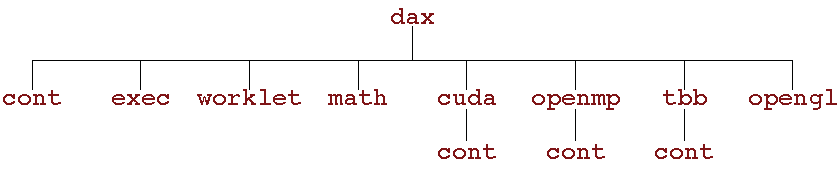
\includegraphics{images/PackageHierarchy}
  \caption{Dax package hierarchy.}
  \label{fig:Packages}
\end{figure}

By convention all classes will be defined in a file with the same name as
the class name (with a \textfilename{.h} extension) located in a directory
corresponding to the package name. For example, the \daxcont{ArrayHandle}
class is found in the \daxheader{dax/cont}{ArrayHandle.h} header. There
are, however, exceptions to this rule. Some smaller classes and types are
grouped together for convienience. These exceptions will be noted as
necessary.

Within each namespace there may also
be \textnamespace{internal}\indexnamespaceone{internal}
and \textnamespace{detail}\indexnamespaceone{detail}
sub-namespaces. The \textnamespace{internal} namespaces contain features
that are used internally and may change without
notice. The \textnamespace{detail} namespaces contain features that are
used by a particular class but must be declared outside of that
class. Users should generally ignore classes in these namespaces.

\index{packages|)}


\section{Basic Provisions}
\label{sec:BasicProvisions}

This section describes the core facilities provided by the Dax
toolkit. These include macros, types, and classes that define the
environment in which code is run, the core types of data stored, and
template introspection.

\subsection{Function and Method Exports}
\label{sec:FunctionAndMethodExports}

Any function or method defined by the Dax toolkit must come with an export
modifier that determines in which environments the function may be
run. These export modifiers are C macros that Dax uses to instruct the
compiler for which architectures to compile each method. Most user code
outside of the Dax toolkit need not use these macros with the important
exception of any classes passed to the Dax toolkit. This occurs when
defining new worklets, array containers, and device adapters.

Dax provides three export macros, \daxcontexport, \daxexecexport, and
\daxexeccontexport, which are used to declare functions and methods that
can run in the control environment, export environment, and both
environments, respectively. These macros get defined by including just
about any Dax header file, but including \daxheader{dax}{Types.h} will
ensure they are defined. 

The export macro is place after the template declaration, if there is one,
and before the return type for the function. Here is a simple example of a
function that will square a value. Since most types you would use this
function on have operators in both the control and execution environments,
the function is exported to both places.

\begin{daxexample}{Usage of export macro.}
template<class ValueType>
DAX_EXEC_CONT_EXPORT
ValueType Square(const ValueType &inValue)
{
 return inValue * inValue;
}
\end{daxexample}

The primary function of the export macros is to interject compiler-specific
keywords that specify what architecture to compile code for. For example,
when compiling with CUDA\index{CUDA}, the control exports have
\textcode{\_\_host\_\_} in them and execution exports have
\textcode{\_\_device\_\_} in them.

There is one additional export macro that is not used for functions but
rather used when declaring a constant data object that is used in the
execution environment. This macro is named
\daxmacro{DAX\_EXEC\_CONSTANT\_EXPORT}\index{export!constant}\index{constant~export}
and is used to declare a constant lookup table used when executing a
worklet. Its primary reason for existing is to add a
\textcode{\_\_constant\_\_} keyword when compiling with CUDA. This export
currently has no effect on any other compiler.

\subsection{Core Data Types}
\label{sec:CoreDataTypes}

Except in rare circumstances where precision is not a concern, the Dax
toolkit does not directly use the core C types like \textcode{int},
\textcode{float}, and \textcode{double}. Instead, Dax provides its own core
types, which are declared in \daxheader{dax}{Types.h}.

\subsubsection{Single Number Types}

All floating point values should be declared as type \dax{Scalar}, and all
integer values, generally used for indexing, should be declared as type
\dax{Id}. The chief advantage of using these declared types rather than the
core C types is that the precision can easily be changed. By default, both
types are 32 bits wide. The CMake configuration options
\cmakevar{DAX\_USE\_DOUBLE\_PRECISION} and \cmakevar{DAX\_USE\_64BIT\_IDS}
can be used to change the \dax{Scalar} type and \dax{Id} type,
respectively, to be 64 bits wide. The configuration can be overridden by
defining the C macro \daxmacro{DAX\_USE\_DOUBLE\_PRECISION} or
\daxmacro{DAX\_NO\_DOUBLE\_PRECISION} to force \dax{Scalar} to be either 64
or 32 bits and defining the C macro \daxmacro{DAX\_USE\_64BIT\_IDS} or
\daxmacro{DAX\_NO\_64BIT\_IDS} to force \dax{Id} to be either 64 or 32
bits. These macros must be defined before any Dax header files are included
to take effect. For convenience, you can include either
\daxheader{dax/internal}{ConfigureFor32.h} or
\daxheader{dax/internal}{ConfigureFor64.h} to force both \dax{Scalar} and
\dax{Id} to be 32 or 64 bits. The reason Dax uses macros to determine these
type widths rather than templates is to reduce the number of template
parameters required in the already template-heavy Dax classes and
functions.

\subsubsection{Vector Types}

Visualization algorithms also often require operations on short
vectors. Arrays indexed in up to three dimensions are common. Data is often
defined in 2-space and 3-space, and transformations are typically done in
homogeneous coordinates of length 4. To simplify these types of operations,
Dax provides several vector data types.

The types \dax{Id2} and \dax{Id3} are couple and triple values of type
\dax{Id}. The types \dax{Vector2}, \dax{Vector3}, and \dax{Vector4} are
couple, triple, and quadruple values of type \dax{Scalar}. The elements of
these vectors are accessed with the bracket operator, so they syntatically
appear like short arrays. They additionally have a constant named
\textidentifier{NUM\_COMPONENTS}\index{NUM\_COMPONENTS} to specify how many
components are in the tuple.

The default constructor of these vector types leaves the values
uninitialized. All vectors have a constructor with one arguments that is
used to initialize all components. All these vectors also have a
constructor that allows you to set the individual components. Likewise,
there are a set of \dax{make\_Id*} and \dax{make\_Vector*} functions that
build initialized vector types.

\begin{daxexample}{Creating vector types.}
dax::Vector3 A(1);                      // A is {1, 1, 1}
A[1] = 2;                               // A is now {1, 2, 1}
dax::Vector3 B(1, 2, 3);                // B is {1, 2, 3}
dax::Vector3 C = make_Vector3(3, 4, 5); // C is {3, 4, 5}
\end{daxexample}

The vector types all support component-wise arithmetic using the operators
for plus (\textcode{+}), minus (\textcode{-}), multiply (\textcode{*}), and
divide (\textcode{/}). They also support scalar to vector multiplication
with the multiply operator. The comparison operators equal (\textcode{==})
is true if every pair of corresponding components are true and not equal
(\textcode{!=}) is true otherwise.  A special \dax{dot} function is
overloaded to provide a dot product for every type of vector.

\begin{daxexample}{Vector operations.}
dax::Vector3 A(1, 2, 3);
dax::Vector3 B(4, 5, 6.5);
dax::Vector3 C = A + B;                     // C is {5, 7, 9.5}
dax::Vector3 D = 2 * C;                     // D is {10, 14, 19}
dax::Scalar s = dax::dot(A, B);             // s is 33.5
bool b1 = (A == B);                         // b1 is false
bool b2 = (A == dax::make_Vector3(1, 2, 3); // b2 is true
\end{daxexample}

\subsubsection{Tuple}

The Dax toolkit provides the templated class \dax{Tuple}\tparams{T,Size},
which is essentially a fixed length array of a given type. \dax{Tuple}
objects behave just like the vector types previously described but with any
type and length that you specify.

\begin{daxexample}{The tuple class.}
dax::Tuple<dax::Scalar, 5> A(2);  // A is {2, 2, 2, 2, 2}
for (int index = 1; index < NUM_COMPONENTS; index++)
  {
  A[index] = A[index-1] * 1.5;
  }
// A is now {2, 3, 4.5, 6.75, 10.125}
\end{daxexample}

The same operators that work on the vector types work on \dax{Tuple} with
the caveat that the operator must work on the component type of the
tuple. For example, the multiply operator will work fine on objects of type
\dax{Tuple}\tparams{char,3}, but the multiply operator will not work on objects
of type \dax{Tuple}\tparams{std::string,3} because you cannot multiply
objects of type \textcode{std::string}.

A \dax{Tuple} of the appropriate type can be used interchangeably with a
matching vector type. In fact, a vector type is really just a typedef over
a \dax{Tuple}. This is convienient for a number of things including writing
generic functions that work over all types.

\begin{daxexample}{Interchangeability of tuples and vector types.}
template<typename T, int Size>
DAX_EXEC_CONT_EXPORT
T SumComponents(const dax::Tuple<T,Size> &tuple)
{
  T result = tuple[0];
  for (int index = 1; index < Size; index++)
    {
    result += tuple[index];
    }
  return result;
}

void Foo()
{
  dax::Id a = SumComponents(dax::make_Id3(1, 2, 3));                    // a is 6
  dax::Scalar b = SumComponents(dax::make_Vector4(1.5, 2.5, 3.5, 4.5)); // b is 12
}
\end{daxexample}

In addition to generalizing vector operations and making arbitrarily long
vectors, \dax{Tuple} is useful for creating any sequence of homogeneous
objects. Here is a simple example of using \dax{Tuple} to hold the state of
a polygon.

\begin{daxexample}{Usage of a tuple.}
dax::Tuple<dax::Vector2,3> equilateralTriange(dax::make_Vector2(0.0, 0.0),
                                              dax::make_Vector2(1.0, 0.0),
                                              dax::make_Vector2(0.5, 0.866));
\end{daxexample}

\subsubsection{Extents}

\dax{Extent3} is a simple structure that holds the extent information for
structured data (data defined on a regular grid). It contains to \dax{Id3}
fields named \textcode{Min} and \textcode{Max} that define the minimum and
maximum. \dax{Extent3} and several associated helper functions are defined
in the \daxheader{dax}{Extent.h} header.

\begin{daxexample}{Creating and using an \textidentifier{Extent3}.}
#include <dax/Extent.h>
#include <dax/Types.h>

void ExtentExample()
{
  // Make an extent that defines a grid that has 5x5x3 points and "centered"
  // at index (0,0,0).
  dax::Extent3 extent(dax::make_Id3(-2,-2,-1), dax::make_Id3(2,2,1));

  dax::Id3 minIndices = extent.Min; // Is (-2,-2,-1)
  dax::Id3 maxIndices = extent.Max; // Is (2,2,1)

  dax::Id3 pointDimensions = extentDimensions(extent); // Returns (5,5,3)
  dax::Id3 cellDimensions = extentCellDimensions(extent); // Returns (4,4,2)

  dax::Id3 pointIndexA = flatIndexToIndex3(31, extent); // Returns (-1,-1,0)
  dax::Id3 cellIndexA = flatIndexToIndex3Cell(31, extent); // Returns (1,1,0)

  dax::Id pointIndexB = index3ToFlatIndex(dax::make_Id3(2,-1,0), extent); // Returns 34
  dax::Id pointIndexB = index3ToFlatIndexCell(dax::make_Id(2,-1,0), extent); // Returns 24
}
\end{daxexample}

\subsubsection{Pair}

The Dax toolkit defines a \dax{Pair}\tparams{T1,T2} templated object that
behaves just like \textcode{std:\colonhyp{}pair} from the standard template
library. The difference is that \dax{Pair} will work in both the execution
and control environment, whereas the STL \textcode{std::pair} does not
always work in the execution environment.

The Dax version of \dax{Pair} supports the same types, fields, and
operations as the STL version. Dax also provides a \dax{make\_Pair}
function for convenience.

\subsection{Traits}
\label{sec:Traits}

\index{traits|(}

When using templated types, it is often necessary to get information about
the type or specialize code based on general properties of the type. The
Dax toolkit uses traits classes to publish and retreive information about
types. A traits class is simply a templated structure that provides
typedefs for tag\index{tag} structures, empty types used for
identification. The traits classes might also contain constant numbers and
helpful static functions. See Mayers\scite{Mayers2009} for a description of
traits classes and their uses.

\subsubsection{Type Traits}

The \dax{TypeTraits}\tparams{T} templated class provides basic information
about a core type. These type traits are available for all the basic C++
types as well as the core Dax types described in
Section~\ref{sec:CoreDataTypes}. \dax{TypeTraits} contains the following
elements.

\begin{description}
\item[\textidentifier{NumericTag}] \index{NumericTag} This type is set to
  either \dax{TypeTraitsRealTag} or \dax{TypeTraitsIntegerTag} to signal
  that the type represents either floating point numbers or integers.
\item[\textidentifier{DimensionalityTag}] \index{DimensionalityTag} This
  type is set to either \dax{TypeTraitsScalarTag} or
  \dax{TypeTraitsVectorTag} to signal that the type represents either a
  single scalar value or a tuple of values.
\end{description}

The definition of \dax{TypeTraits} for \dax{Scalar} could like something
like this.
\begin{daxexample}{Definition of \protect \dax{TypeTraits}\tparams{\protect \dax{Scalar}}.}
namespace dax {

template<>
struct TypeTraits<dax::Scalar>
{
  typedef TypeTraitsRealTag NumericTag;
  typedef TypeTraitsScalarTag DimensionalityTag;
};

}
\end{daxexample}

Here is a simple example of using \dax{TypeTraits} to implement a generic
function that behaves like the modulus operator (\textcode{\%}) for all
types including floating points and vectors.

\begin{daxexample}[ex:TypeTraits]{Using \textidentifier{TypeTraits} for a generic modulus.}
#include <dax/TypeTraits.h>

template<typename T>
T Modulus(const T &numerator, const T &denominator);

namespace detail {

template<typename T>
T ModulusImpl(const T &numerator,
              const T &denominator,
              dax::TypeTraitsIntegerTag,
              dax::TypeTraitsScalarTag)
{
  return numerator % denominator;
}

template<typename T>
T ModulusImpl(const T &numerator,
              const T &denominator,
              dax::TypeTraitsRealTag,
              dax::TypeTraitsScalarTag)
{
  T quotient = numerator / denominator;
  return (quotient - dax::math::Floor(quotient))*demoninator;
}

template<typename T, typename NumericTag>
T ModulusImpl(const T &numerator,
              const T &denominator,
              NumericTag,
              dax::TypeTraitsVectorTag)
{
  T result;
  for (int componentIndex = 0; componentIndex < T::NUM_COMPONENTS; componentIndex++)
    {
    result[componentIndex] = Modulus(numerator[componentIndex],denominator[componentIndex]);
    }
}

} // namespace detail

template<typename T>
T Modulus(const T &numerator, const T &denominator)
{
  return detail::ModulusImpl(numerator,
                             denominator,
                             typename dax::TypeTraits<T>::NumericTag(),
                             typename dax::TypeTraits<T>::DimensionalityTag());
}
\end{daxexample}

\subsubsection{Vector Traits}

The \dax{VectorTraits}\tparams{T} templated class provides information and
accessors to vector and tuple types. It contains the following elements.

\begin{description}
\item[\textidentifier{ComponentType}] \index{ComponentType} This type is
  set to the type for each component in the vector. For example, a
  \dax{Vector3} has \textidentifier{ComponentType} defined as \dax{Scalar}.
\item[\textidentifier{NUM\_COMPONENTS}] \index{NUM\_COMPONENTS} An integer
  specifying how many components are contained in the vector.
\item[\textidentifier{HasMultipleComponents}] \index{HasMultipleComponents}
  This type is set to either \dax{VectorTraitsTagSingleComponent} if the
  vector length is size 1 or \dax{VectorTraitsTagMultipleComponents}
  otherwise. This tag can be useful for creating specialized functions when
  a vector is really just a scalar.
\item[\textcode{GetComponent}] \index{GetComponent} A static method that
  takes a vector and returns a particular component.
\item[\textcode{SetComponent}] \index{SetComponent} A static method that
  takes a vector and sets are particular component to a given value.
\item[\textcode{ToTuple}] \index{ToTuple} A static method that converts a
  vector of the given type to a \dax{Tuple}.
\end{description}

The definition of \dax{VectorTraits} for \dax{Id3} could like something
like this.
\begin{daxexample}{Definition of \protect \dax{VectorTraits}\tparams{\protect \dax{Id3}}.}
template<>
struct VectorTraits<dax::Id3>
{
  typedef dax::Id ComponentType;
  static const int NUM_COMPONENTS = 3;
  typedef VectorTraitsTagMultipleComponents HasMultipleComponents;

  DAX_EXEC_CONT_EXPORT
  static dax::Id &GetComponent(dax::Id3 &vector, int component) {
    return vector[component];
  }

  DAX_EXEC_CONT_EXPORT
  static void SetComponent(dax::Id3 &vector, int component, dax::Id value) {
    vector[component] = value;
  }

  DAX_EXEC_CONT_EXPORT
  static dax::Tuple<dax::Id,3> ToTuple(const dax::Id3 &vector) {
    return vector;
  }
};
\end{daxexample}

The real power of vector traits is that they simplify creating generic
operations on any type that can look like a vector. This includes
operations on scalar values as if they were vectors of size one. The
following code uses vector traits to simplify the implementation of less
functors\index{less} that define an ordering that can be used for sorting
and other operations.

\begin{daxexample}{Using \textidentifier{VectorTraits} for less functors.}
#include <dax/VectorTraits.h>

// This functor provides a total ordering of vectors. Every compared vector
// will be either less, greater, or equal.
template<typename T>
struct LessTotalOrder
{
  bool operator()(const T &left, const T &right)
  {
    for (int index = 0; index < dax::VectorTraits<T>::NUM_COMPONENTS; index++)
      {
      const T &leftValue = dax::VectorTraits<T>::GetComponent(left, index);
      const T &rightValue = dax::VectorTraits<T>::GetComponent(right, index);
      if (leftValue < rightValue) { return true; }
      if (rightValue < leftValue) { return false; }
      }
    // If we are here, the vectors are equal.
    return false;
  }
};

// This functor provides a partial ordering of vectors. It returns true if and
// only if all components satisfy the less operation. It is possible for
// vectors to be neither less, greater, nor equal, but the transitive closure
// is still valid.
template<typename T>
struct LessTotalOrder
{
  bool operator()(const T &left, const T &right)
  {
    for (int index = 0; index < dax::VectorTraits<T>::NUM_COMPONENTS; index++)
      {
      const T &leftValue = dax::VectorTraits<T>::GetComponent(left, index);
      const T &rightValue = dax::VectorTraits<T>::GetComponent(right, index);
      if (!(leftValue < rightValue)) { return false; }
      }
    // If we are here, all components satisfy less than relation.
    return true;
  }
};
\end{daxexample}

\index{traits|)}

%TODO: Document vector operations


\section{Provided Worklets}
\label{sec:ProvidedWorklets}

The Dax toolkit provides several common visualization algorithms
encapsulated in worklets\index{worklet} that can be executed in parallel on
your data. This section describes each of the worklets provided. All
worklets provided by Dax are in the \daxworklet{} namespace and defined in
header files in the \textfilename{dax/worklet} directory.

Much of the support structures for defining data and executing jobs, which
you will see in examples, is defined in the Dax control
environment\index{control~environment}. These features are documented in
Section~\ref{sec:ControlEnvironment}. The Dax toolkit also provides
facilities to make it easy to define your own worklet. Descriptions of
these features are in Section~\ref{sec:ExecutionEnvironment}.

\subsection{Cell Average}
\label{sec:worklet:CellAverage}

The \daxworklet{CellAverage} worklet takes a topology and a field and
averages the value of the field in each point. For each cell, it find the
field value on each point of the cell and takes the average of
those. \daxworklet{CellAverage} is a cheap but inaccurate way to integrate
the value of a field in each cell. A similar worklet named point data to
cell data does a similar operation except that it interpolates the field
value to the parametric center of the cell
(Section~\ref{sec:worklet:PointDataToCellData}), which may be different
than a simple average.

\begin{daxexample}{Cell average worklet.}
#include <dax/worklet/CellAverage.h>

#include <dax/cont/ArrayHandle.h>
#include <dax/cont/Scheduler.h>

template<typename GridType>
DAX_CONT_EXPORT
void RunCellAverage(const GridType &grid,
                    const dax::cont::ArrayHandle<dax::Scalar> &inPointData,
                    dax::cont::ArrayHandle<dax::Scalar> &outCellData)
{
  dax::cont::Scheduler<> scheduler;
  scheduler.Invoke(dax::worklet::CellAverage(), grid, inPointData, outCellData);
}
\end{daxexample}

\subsection{Cell Data to Point Data}

The cell data to point data worklet finds all cells incident on each point
and then averages the field values of all incident cells to the point.

\fix{TODO: Running this worklet needs to be similfied. The scheduler needs
  to be cleaned up to remove the helper classes. Also, there should
  probably be a specialized worklet type for doing cell to point
  operations.}

Running the cell data to point data worklet is a two step process. In the
first step, \daxworklet{CellDataToPointDataGenerateKeys} extracts point
indices for each cell and attaches field values to them. In the second
step, \daxworklet{CellDataToPointDataReduceKeys} collects field values on a
point and averages them.

\begin{daxexample}{Cell data to point data worklet.}
#include <dax/worklet/CellDataToPointData.h>

#include <dax/cont/ArrayHandle.h>
#include <dax/cont/ArrayHandleConstant.h>
#include <dax/cont/GenerateKeysValues.h>
#include <dax/cont/ReduceKeysValues.h>
#include <dax/cont/Scheduler.h>

#include <dax/CellTraits.h>

template<typename GridType, typename FieldType>
DAX_CONT_EXPORT
void RunCellDataToPointData(const GridType &grid,
                            const dax::cont::ArrayHandle<FieldType> &inPointData,
                            dax::cont::ArrayHandle<FieldType> &outCellData)
{
  dax::cont::ArrayHandleConstant<dax::Id> keyGenCounts =
      dax::cont::make_ArrayHandleConstant<dax::Id>(
            dax::CellTraits<CellTag>::NUM_VERTICES, grid.GetNumberOfCells());  

  dax::cont::Scheduler<> scheduler;

  dax::cont::GenerateKeysValues<
      dax::worklet::CellDataToPointDataGenerateKeys,
      dax::cont::ArrayHandleConstant<dax::Id> > generateKeys(keyGenCounts);

  dax::cont::ArrayHandle<dax::Id> keyArray;
  dax::cont::ArrayHandle<FieldType> valueArray;

  scheduler.Invoke(generateKeys, grid, inPointData, keyArray, valueArray);

  dax::cont::ReduceKeysValues<
    dax::worklet::CellDataToPointDataReduceKeys,
    dax::cont::ArrayHandle<dax::Id> > reduceKeys(keyArray);

  scheduler.Invoke(reduceKeys, valueArray, outCellData);
}
\end{daxexample}

\subsection{Cell Gradient}

The \daxworklet{CellGradient} worklet computes the gradient of a point
field at the parametric center of each cell.

\begin{daxexample}{Cell gradient worklet.}
#include <dax/worklet/CellGradient.h>

#include <dax/cont/ArrayHandle.h>
#include <dax/cont/Scheduler.h>

template<typename GridType>
DAX_CONT_EXPORT
void RunCellGradient(const GridType &grid,
                     const dax::cont::ArrayHandle<dax::Scalar> &inPointField,
                     dax::cont::ArrayHandle<dax::Vector3> &outCellGradient)
{
  dax::cont::Scheduler<> scheduler;
  scheduler.Invoke(dax::worklet::CellGradient(),
                   grid,
                   grid.GetPointCoordinates(),
                   inPointField,
                   outCellGradient);
}
\end{daxexample}

\subsection{Cosine}

The \daxworklet{Cosine} worklet computes the cosine of a field. The field
can be either a point field or a cell field (or really, just any array).

\begin{daxexample}{Cosine worklet.}
#include <dax/worklet/Cosine.h>

#include <dax/cont/ArrayHandle.h>
#include <dax/cont/Scheduler.h>

template<typename FieldType>
DAX_CONT_EXPORT
void RunCosine(const dax::cont::ArrayHandle<FieldType> &inField,
               dax::cont::ArrayHandle<FieldType> &outField)
{
  dax::cont::Scheduler<> scheduler;
  scheduler.Invoke(dax::worklet::Cosine(), inField, outField);
}
\end{daxexample}

\subsection{Elevation}

The \daxworklet{Elevation} worklet find the elevation of points in
$\mathrm{R}^3$ in relation to a base plane. The orientation of the
elevation is determined by a low point location and a high point
location. Values lower than the low point and higher than the high point
are clamped to the minimum and maximum values. The range of valid values
can also be specified.

The elevation worklet is design to be run on the point coordinates of a
grid, but in fact could be run on any field or array.

The following example demonstrates finding the elevation of points in a
data set oriented along the x axis. Points between $x=-1$ and $x=1$ are
considered. The scale and bias is set to give the distance from the origin
along the x-axis in the positive direction.

\begin{daxexample}[ex:Elevation]{Elevation worklet.}
#include <dax/worklet/Elevation.h>

#include <dax/cont/ArrayHandle.h>
#include <dax/cont/Scheduler.h>

template<typename GridType>
DAX_CONT_EXPORT
void Elevation(const GridType &grid,
               dax::cont::ArrayHandle<dax::Scalar> &outPointElevation)
{
  dax::worklet::Elevation elevation(dax::make_Vector3(-1.0, 0.0, 0.0),
                                    dax::make_Vector3(1.0, 0.0, 0.0),
                                    dax::make_Vector2(-1.0, 1.0));

  dax::cont::Scheduler<> scheduler;
  scheduler.Invoke(elevation, grid.GetPointCoordinates(), outPointElevation);
}
\end{daxexample}

\subsection{Magnitude}

The \daxworklet{Magnitude} worklet computes the magnitude of a field of
vectors. The field can be either a point field or a cell field (or really,
just any array).

\begin{daxexample}{Magnitude worklet.}
#include <dax/worklet/Magnitude.h>

#include <dax/cont/ArrayHandle.h>
#include <dax/cont/Scheduler.h>

DAX_CONT_EXPORT
void RunMagnitude(const dax::cont::ArrayHandle<dax::Vector3> &inField,
                  dax::cont::ArrayHandle<dax::Scalar> &outField)
{
  dax::cont::Scheduler<> scheduler;
  scheduler.Invoke(dax::worklet::Magnitude(), inField, outField);
}
\end{daxexample}

\subsection{Marching Cubes}

The Marching Cubes worklet takes a volume and extracts the contour surface
where a field value is equal to a given value.

\fix{TODO: Running this worklet needs to be simplified. The scheduler needs
  to be cleaned up to remove the helper classes.}

Running the Marching Cubes worklet is a two step process. In the first
step, \daxworklet{MarchingCubesClassify} identifies how many polygons are
going to be generated for every input cell. In the second step,
\daxworklet{MarchingCubesGenerate} creates the triangles that make up the
surface.

\begin{daxexample}{Marching Cubes worklet.}
#include <dax/worklet/MarchingCubes.h>

#include <dax/cont/ArrayHandle.h>
#include <dax/cont/GenerateInterpolatedCells.h>
#include <dax/cont/Scheduler.h>
#include <dax/cont/UnstructuredGrid.h>

template<typename GridType>
DAX_CONT_EXPORT
void RunMarchingCubes(const GridType &inGrid,
                      const dax::cont::ArrayHandle<FieldType> &inPointData,
                      dax::Scalar isovalue,
                      dax::cont::UnstructuredGrid<dax::CellTagTriangle> &outGrid)
{
  dax::cont::Scheduler<> scheduler;

  dax::cont::ArrayHandle<dax::Id> classification;
  scheduler.Invoke(dax::worklet::MarchingCubesClassify(isovalue),
                   inGrid,
                   inPointData,
                   classification);

  dax::cont::GenerateInterpolatedCells<
    dax::worklet::MarchingCubesGenerate, dax::cont::ArrayHandle<dax::Id> >
        generate(dax::worklet::MarchingCubesGenerate(isovalue), classification);
  scheduler.Invoke(generate, inGrid, outGrid, inPointData);
}
\end{daxexample}

\subsection{Point Data to Cell Data}
\label{sec:worklet:PointDataToCellData}

The \daxworklet{PointDataToCellData} worklet takes a topology and a field
and averages the value of the field in each point. For each cell, it
interpolates a point field to the center of the cell. A similar worklet
named cell average does a similar operation except that simply averages the
field values (Section~\ref{sec:worklet:CellAverage}), which may be
different than the interpolation.

The following example uses \daxworklet{PointDataToCellData} to find the
coordinates of each cell center.

\begin{daxexample}{Point data to cell data worklet.}
#include <dax/worklet/PointDataToCellData.h>

#include <dax/cont/ArrayHandle.h>
#include <dax/cont/Scheduler.h>

template<typename GridType>
DAX_CONT_EXPORT
void RunPointDataToCellData(const GridType &grid,
                            dax::cont::ArrayHandle<dax::Scalar> &outCellCenters)
{
  dax::cont::Scheduler<> scheduler;
  scheduler.Invoke(dax::worklet::PointDataToCellData(),
                   grid,
                   grid.GetPointCoordinates(),
                   Centers);
}
\end{daxexample}

\subsection{Sine}

The \daxworklet{Sine} worklet computes the sine of a field. The field
can be either a point field or a cell field (or really, just any array).

\begin{daxexample}{Sine worklet.}
#include <dax/worklet/Sine.h>

#include <dax/cont/ArrayHandle.h>
#include <dax/cont/Scheduler.h>

template<typename FieldType>
DAX_CONT_EXPORT
void RunSine(const dax::cont::ArrayHandle<FieldType> &inField,
             dax::cont::ArrayHandle<FieldType> &outField)
{
  dax::cont::Scheduler<> scheduler;
  scheduler.Invoke(dax::worklet::Sine(), inField, outField);
}
\end{daxexample}

\subsection{Slice}

The slice worklet takes a volume and intersects it with a plane.

\fix{TODO: Running this worklet needs to be simplified. The scheduler needs
  to be cleaned up to remove the helper classes.}

Running the slice worklet is a two step process. In the first step,
\daxworklet{SliceClassify} identifies how many polygons are going to be
generated for every input cell. In the second step,
\daxworklet{SliceGenerate} creates the triangles that make up the surface
that is the intersection of the volume and the plane.

\begin{daxexample}{Slice worklet.}
#include <dax/worklet/Slice.h>

#include <dax/cont/ArrayHandle.h>
#include <dax/cont/GenerateInterpolatedCells.h>
#include <dax/cont/Scheduler.h>
#include <dax/cont/UnstructuredGrid.h>

template<typename GridType>
DAX_CONT_EXPORT
void RunSlice(const GridType &inGrid,
              const dax::cont::ArrayHandle<FieldType> &inPointData,
              dax::Scalar isovalue,
              dax::cont::UnstructuredGrid<dax::CellTagTriangle> &outGrid)
{
  dax::cont::Scheduler<> scheduler;

  dax::cont::ArrayHandle<dax::Id> classification;
  scheduler.Invoke(dax::worklet::SliceClassify(isovalue),
                   inGrid,
                   inPointData,
                   classification);

  dax::cont::GenerateInterpolatedCells<
    dax::worklet::SliceGenerate, dax::cont::ArrayHandle<dax::Id> >
        generate(dax::worklet::SliceGenerate(isovalue), classification);
  scheduler.Invoke(generate, inGrid, outGrid, inPointData);
}
\end{daxexample}

\subsection{Square}

The \daxworklet{Square} worklet computes the square of all the values in a
field. (It finds a component-wise square in the case of vector types.) The
field can be either a point field or a cell field (or really, just any
array).

\begin{daxexample}{Square worklet.}
#include <dax/worklet/Square.h>

#include <dax/cont/ArrayHandle.h>
#include <dax/cont/Scheduler.h>

template<typename FieldType>
DAX_CONT_EXPORT
void RunSquare(const dax::cont::ArrayHandle<FieldType> &inField,
               dax::cont::ArrayHandle<FieldType> &outField)
{
  dax::cont::Scheduler<> scheduler;
  scheduler.Invoke(dax::worklet::Square(), inField, outField);
}
\end{daxexample}

\subsection{Tetrahedralize}

The \daxworklet{Tetrahedralize} takes a data set and divides each cell into
a group of simplicies (tetrahedra) that comprise the volume.

\fix{TODO: Running this worklet needs to be simplfied. The scheduler needs
  to be cleaned up to remove the helper classes. There is also some
  hinkiness involved with specifing the count (classification) array.}

\begin{daxexample}{Tetrahedralize worklet.}
#include <dax/worklet/Tetrahedralize.h>

#include <dax/cont/ArrayHandleConstant.h>
#include <dax/cont/GenerateTopology.h>
#include <dax/cont/Scheduler.h>
#include <dax/cont/UnstructuredGrid.h>

template<typename GridType>
DAX_CONT_EXPORT
void RunTetrahedralize(const GridType &inGrid,
                       dax::cont::UnstructuredGrid<dax::CellTagTetrahedron> &outGrid)
{
  typedef dax::cont::ArrayHandleConstant<dax::Id> ClassificationType;
  ClassificationType classification(5, inGrid.GetNumberOfCells());

  dax::cont::GenerateTopology<dax::worklet::Tetrahedralize,ClassificationType>
      generate(classification);
  generate.SetRemoveDuplicatePoints(false);

  dax::cont::Scheduler<> scheduler;
  scheduler.Invoke(generate, inGrid, outGrid);
}
\end{daxexample}

\subsection{Threshold}

The threshold worklet takes a grid and extracts all cells with field values
within a range specified by a minimum and maximum value.

\fix{TODO: Running this worklet needs to be simplified. The scheduler needs
  to be cleaned up to remove the helper classes.}

Running the threshold worklet is a two step process. In the first step,
\daxworklet{ThresholdClassify} identifies how many cells are going to be
generated for every input cell (0 or 1). In the second step,
\daxworklet{ThresholdTopology} creates a new grid with the passed cells.

\begin{daxexample}{Threshold worklet.}
#include <dax/worklet/Threshold.h>

#include <dax/cont/ArrayHandle.h>
#include <dax/cont/GenerateTopology.h>
#include <dax/cont/Scheduler.h>
#include <dax/cont/UnstructuredGrid.h>

template<typename CellType, typename FieldType>
DAX_CONT_EXPORT
void RunThreshold(const dax::cont::UnstructuredGrid<CellType> &inGrid,
                  const dax::cont::ArrayHandle<FieldType> &inPointField,
                  FieldType thresholdMin,
                  FieldType thresholdMax,
                  dax::cont::UnstructuredGrid<CellType> &outGrid,
                  dax::cont::ArrayHandle<FieldType> &outPointField)
{
  dax::cont::Scheduler<> scheduler;
  
  typedef dax::cont::ArrayHandle<dax::Id> ClassificationType;
  ClassificationType classification;

  scheduler.Invoke(dax::worklet::ThresholdClassify<FieldType>(thresholdMin, thresholdMax),
                   inGrid,
                   inPointField,
                   classification);

  dax::cont::GenerateTopology<dax::worklet::ThresholdTopology,ClassificationType>
      generate(classification);

  scheduler.Invoke(generate, inGrid, outGrid);

  generate.CompactPointField(inPointField, outPointField);
}
\end{daxexample}


\section{Control Environment}
\label{sec:ControlEnvironment}

\index{control~environment|(}

The control environment is where code that interfaces with applications and
I/O devices. The associated API is designed for users that want to use the
Dax toolkit to analyze their data using provided or supplied worklets. Code
for the control environment is designed to run on a single thread (or one
single thread per process in an MPI job).

Most users of the Dax toolkit will have some interaction with the Dax
toolkit, for you cannot define data sturctures or execute any algorithms
without it.

\subsection{Device Adapter Tag}
\label{sec:DeviceAdapterTag}

\index{device~adapter|(}

The Dax toolkit uses a feature called a device adapter to define what type
of device will be used to run algorithms. The device adapter encapsulates
the device-specific code required to port to various devices. More
information on the function of the device adapter are given in
Section~\ref{sec:DeviceIndependence}.

The device adapter is identified by a \keyterm{device adapter tag}.
\index{device~adapter~tag} This tag, which is simply an empty struct type,
is used as the template parameter for several classes in the Dax control
environment and causes these classes to direct their work to a particular
device.

There are two ways to select a device adapter. The first is to make a
global selection of a default device adapter. The second is to specify a
specific device adapter as a template parameter.

\subsubsection{Default Device Adapter}

A default device adapter tag is specified in
\daxheader{dax/cont}{DeviceAdapter.h} (although it can also by specified in
many other Dax headers via header dependencies). If no other information is
given, Dax attempts to choose a default device adapter that is a best fit
for the system it is compiled on. Dax currently select the default device
adapter with the following sequence of conditions.

\begin{itemize}
\item \index{CUDA} If the source code is being compiled by CUDA, the CUDA
  device is used.
\item \index{OpenMP} If the CUDA compiler is not being used and the current
  compiler supports OpenMP, then the OpenMP device is used.
\item \index{Intel Threading Building Blocks} \index{TBB} If the compiler
  supports neither CUDA nor OpenMP and the Dax Toolkit was configured to
  use Intel Threading Building Blocks, then that device is used.
\item \index{serial} If no parallel device adapters are found, then the Dax
  Toolkit falls back to a serial device.
\end{itemize}

You can also set the default device adapter specifically by setting the
\daxmacro{DAX\_DEVICE\_ADAPTER} macro. This macro must be set \emph{before}
including any Dax header files. You can set \daxmacro{DAX\_DEVICE\_ADAPTER}
to any one of the following.

\begin{description}
\item[\daxmacro{DAX\_DEVICE\_ADAPTER\_SERIAL}] Performs all computation on
  the same single thread as the control environment. This device is useful
  for debugging. This device is always available.
\item[\daxmacro{DAX\_DEVICE\_ADAPTER\_CUDA}] Uses a CUDA capabile GPU
  device. For this device to work, Dax must be configured to use CUDA and
  the code must be compiled by the CUDA \textfilename{nvcc} compiler.
\item[\daxmacro{DAX\_DEVICE\_ADAPTER\_OPENMP}] Uses OpenMP compiler
  extensions to run algorithms on multiple threads. For this device to
  work, Dax must be configured to use OpenMP and the code must be compiled
  with a compiler that supports OpenMP pragmas.
\item[\daxmacro{DAX\_DEVICE\_ADAPTER\_TBB}] Uses the Intel Threading
  Building Blocks library to run algorithms on multiple threads. For this
  device to work, Dax must be configured to use TBB and the executable must
  be linked to the TBB library.
\end{description}

These macros provide a useful mechanism for quickly reconfiguring code to
run on different devices. The following example shows a typical block of
code at the top of a source file that could be used for quick
reconfigurations.

\begin{daxexample}{Macros to port Dax code among different devices}
// Uncomment one (and only one) of the following to reconfigure the Dax
// code to use a particular device. Comment them all to automaticall pick a
// device.
//#define DAX_DEVICE_ADAPTER DAX_DEVICE_ADAPTER_SERIAL
#define DAX_DEVICE_ADAPTER DAX_DEVICE_ADAPTER_CUDA
//#define DAX_DEVICE_ADAPTER DAX_DEVICE_ADAPTER_OPENMP
//#define DAX_DEVICE_ADAPTER DAX_DEVICE_ADAPTER_TBB

#include <dax/cont/DeviceAdapter.h>
\end{daxexample}

The default device adapter can always be overridden by specifying a device
adapter tag, as described in the next section. There is actually one more
internal default device addapter named
\daxmacro{DAX\_DEVICE\_ADAPTER\_ERROR} that will cause a compile error if
any component attempts to use the default device adapter. This feature is
most often used in testing code to check when device adapters should be
specified.

\subsubsection{Specifying Device Adapter Tags}

In addition to setting a global default device adapter, it is possible to
explicitly set which device adapter to use in any feature provided by
Dax. This is done by providing a device adapter tag as a template argument
to Dax templated objects. The following device adapter tags are available
in Dax.

\begin{description}
\item[\daxcont{DeviceAdapterTagSerial}] \index{serial} Performs all
  computation on the same single thread as the control environment. This
  device is useful for debugging. This device is always available. This tag
  is defined in \daxheader{dax/cont}{DeviceAdapterSerial.h}.
\item[\daxcudacont{DeviceAdapterTagCuda}] \index{CUDA} Uses a CUDA capabile
  GPU device. For this device to work, Dax must be configured to use CUDA
  and the code must be compiled by the CUDA \textfilename{nvcc}
  compiler. This tag is defined in
  \daxheader{dax/cuda/cont}{DeviceAdapterCuda.h}.
\item[\daxopenmpcont{DeviceAdapterTagOpenMP}] \index{OpenMP} Uses OpenMP
  compiler extensions to run algorithms on multiple threads. For this
  device to work, Dax must be configured to use OpenMP and the code must be
  compiled with a compiler that supports OpenMP pragmas. This tag is
  defined in \daxheader{dax/openmp/cont}{DeviceAdapterOpenMP.h}.
\item[\daxtbbcont{DeviceAdapterTagTBB}]
  \index{Intel Threading Building Blocks} \index{TBB} Uses the Intel
  Threading Building Blocks library to run algorithms on multiple
  threads. For this device to work, Dax must be configured to use TBB and
  the executable must be linked to the TBB library. This tag is defined in
  \daxheader{dax/tbb/cont}{DeviceAdapterTBB.h}.
\end{description}

The following example schedules the elevation worklet much like shown in
Example~\ref{ex:Elevation} on page~\pageref{ex:Elevation} but also
specifies using the Intel Threading Building blocks device adapter.
\index{Intel Threading Building Blocks} \index{TBB}
In particular, consider the template parameter of the \daxcont{Scheduler}
class.
\begin{daxexample}{Calling the Elevation worklet with a specific device adapter.}
dax::worklet::Elevation elevation(dax::make_Vector3(-1.0, 0.0, 0.0),
                                  dax::make_Vector3(1.0, 0.0, 0.0),
                                  dax::make_Vector2(-1.0, 1.0));

dax::cont::Scheduler<dax::tbb::cont::DeviceAdapterTagTBB> scheduler;
scheduler.Invoke(elevation, grid.GetPointCoordinates(), outPointElevation);
\end{daxexample}

When structuring your code to always specify a particular device adapter,
consider setting the default device adapter (with the
\daxmacro{DAX\_DEVICE\_ADAPTER} macro) to
\daxmacro{DAX\_DEVICE\_ADAPTER\_ERROR}. This will cause the compiler to
produce an error if any object is instantiated with the default device
adapter, which checks to make sure the code properly specifies every device
adapter parameter.

The Dax toolkit also defines a macro named
\daxmacro{DAX\_DEFAULT\_DEVICE\_ADAPTER\_TAG} that can be used in place of
an explicit device adapter tag to use the default tag. This macro is used
to create new templates that have template parameters for device adapters
that can use the default. The following example has a (rather artificial)
declaration of a helper class for executing the elevation worklet.
\begin{daxexample}{Declaring a template with a default device adapter.}
template<typename DeviceAdapter = DAX_DEFAULT_DEVICE_ADAPTER_TAG>
class MyElevationScheduler
{
public:
  void DoSchedule()
  {
    dax::cont::Scheduler<DeviceAdapter> scheduler;
    scheduler.Invoke(dax::Worklet::Elevation(),
                     this->Grid.GetPointCoordinates(),
                     this->OutPointElevation);
\end{daxexample}

\index{device~adapter|)}

\subsection{Array Handle}
\label{sec:ArrayHandle}

\index{array~handle|(}

An \keyterm{array handle}, implemented with the \daxcont{ArrayHandle}
class, manages an array of data that can be accessed or manipulated by Dax
algorithms. It is typical to construct an array handle in the control
environment to pass data to an algorithm running in the execution
environment. It is also typical for an algorithm running in the execution
environment to allocate and populate an array handle, which can then be
read back in the control environment. It is also possible for an array
handle to manage data created by one Dax algorithm and passed to another,
remaining in the execution environment the whole time and never copied to
the control environment.

The array handle may have up to two copies of the array, one for the
control environment and one for the execution environment. However,
depending on the device and how the array is being used, the array handle
will only have one copy when possible. Copies between the environments are
implicit and lazy. They are copied only when an operation needs data in an
environment where the data is not.

\daxcont{ArrayHandle} behaves like a shared smart pointer in that when the
C++ object is copied, each copy holds a reference to the same array. These
copies are reference counted so that when all copies of the
\daxcont{ArrayHandle} are destroyed, any allocated memory is released.

\subsubsection{Creating Array Handles}

\daxcont{ArrayHandle} is a templated class with three template
parameters. The first template parameter is the only one required and
specifies the base type of the entries in the array. The second template
parameter specifies the container used when storing data in the control
environment. Containers are discussed later in this section, and for now we
will use the default value. The third template parameter is a device
adpater tag that specifies what device is used in the execution
environment. Device adapter tags are described in
Section~\ref{sec:DeviceAdapterTag}. Most of the examples here will use the
default device adapter.

\begin{daxexample}{Declaration of the \protect\daxcont{ArrayHandle} templated class.}
template<
    typename T,
    typename ArrayContainerControlTag = DAX_DEFAULT_ARRAY_CONTAINER_CONTROL_TAG,
    typename DeviceAdapterTag = DAX_DEFAULT_DEVICE_ADAPTER_TAG>
class ArrayHandle;
\end{daxexample}

There are multiple ways to create and populate an array handle. The default
\daxcont{ArrayHandle} constructor will create an empty array with nothing
allocated in either the control or execution environment. This is
convienient for creating arrays used as the output for algorithms.

\begin{daxexample}{Creating an \textidentifier{ArrayHandle} for output data.}
dax::cont::ArrayHandle<dax::Scalar> outputArray;
\end{daxexample}

Constructing an \daxcont{ArrayHandle} that points to a provided C array or
\textcode{std::vector} is straightforward with the
\daxcont{make\_ArrayHandle} functions. These functions will make an array
handle that points to the array data that you provide.

\begin{daxexample}{Creating an \textidentifier{ArrayHandle} that points to a provided C array.}
dax::Scalar dataBuffer[50];
// Populate dataBuffer with meaningful data. Perhaps read data from a file.

dax::cont::ArrayHandle<dax::Scalar> inputArray = dax::cont::make_ArrayHandle(dataBuffer,50);
\end{daxexample}

\begin{daxexample}[ex:ArrayHandleFromVector]{Creating an \textidentifier{ArrayHandle} that points to a provided \textcode{std::vector}.}
std::vector<dax::Scalar> dataBuffer;
// Populate dataBuffer with meaningful data. Perhaps read data from a file.

dax::cont::ArrayHandle<dax::Scalar> inputArray = dax::cont::make_ArrayHandle(dataBuffer);
\end{daxexample}

\emph{Be aware} that \daxcont{make\_ArrayHandle} makes a shallow pointer
copy. This means that if you change or delete the data provided, the
internal state of \daxcont{ArrayHandle} becomes invalid and undefined
behavior can ensue. The most common manifestation of this error happens
when a \textcode{std::vector} goes out of scope. This subtle interaction
will cause the \daxcont{ArrayHandle} to point to an unallocated portion of
the memory heap. For example, if the code in
Example~\ref{ex:ArrayHandleFromVector} where to be placed within a callable
function or method, it could cause the \daxcont{ArrayHandle} to become
invalid.

\begin{daxexample}{Invalidating an \textidentifier{ArrayHandle} by letting the source \textcode{std::vector} leave scope.}
DAX_CONT_EXPORT
dax::cont::ArrayHandle<dax::Scalar> BadDataLoad()
{
  std::vector<dax::Scalar> dataBuffer;
  // Populate dataBuffer with meaningful data. Perhaps read data from a file.

  dax::cont::ArrayHandle<dax::Scalar> inputArray = dax::cont::make_ArrayHandle(dataBuffer);

  return inputArray;
  // THIS IS WRONG! At this point dataBuffer goes out of scope and deletes its memory.
  // However, inputArray has a pointer to that memory, which becomes an invalid pointer
  // in the returned object. Bad things will happen when the ArrayHandle is used.
}

DAX_CONT_EXPORT
dax::cont::ArrayHandle<dax::Scalar> SafeDataLoad()
{
  std::vector<dax::Scalar> dataBuffer;
  // Populate dataBuffer with meaningful data. Perhaps read data from a file.

  dax::cont::ArrayHandle<dax::Scalar> tmpArray = dax::cont::make_ArrayHandle(dataBuffer);

  // This copies the data from one ArrayHandle to another (in the execution environment).
  // Although it is an extraneous copy, it is usually pretty fast on a parallel device.
  // Another option is to make sure that the buffer in the std::vector never goes out
  // of scope before all the ArrayHandle references, but this extra step allows the
  // ArrayHandle to manage its own memory and ensure everything is valid.
  dax::cont::ArrayHandle<dax::Scalar> inputArray;
  dax::cont::DeviceAdapterAlgorithm<DAX_DEFAULT_DEVICE_ADAPTER_TAG>::Copy(
      tmpArray, inputArray);

  return inputArray;
  // This is safe.
}
\end{daxexample}

\subsubsection{Retrieving Data from an Array Handle}

An array handle does not provide direct access to its underlying data by
design. The most straightforward way to get data from an array handle is to
use the \textcode{CopyInto} method. \textcode{CopyInto} takes an
STL-compatible forward iterator and copies all the data into that
iterator. It is assumed that the iterator can be advanced enough to copy
all data into the target array. The number of entries in the array handle
can be retrieved with the \textcode{GetNumberOfValues} method, and the
target array should be at least that big.

\begin{daxexample}[ex:ArrayHandle::CopyInto]{Retrieving \textidentifier{ArrayHandle} data with \textcode{CopyInto}.}
dax::cont::ArrayHandle<dax::Scalar> outArray;
// Do something that fills outArray

std::vector<dax::Scalar> resultBuffer(outArray.GetNumberOfValues());
outArray.CopyInto(resultBuffer.begin());
\end{daxexample}

There are two other ways data can be retrieved from an array handle. The
first is to request an array portal to the data and the second is to define
a new container that points to a particular data structure. Both of these
methods are discussed in more detail in later sections.

\subsubsection{Array Portals}
\label{sec:ArrayPortals}

\index{array~portal|(}

An array handle defines auxiliary structures called \keyterm{array portals}
that provide direct access into its data. An array portal is a simple
object that is somewhat functonally equivalent to an STL-type iterator, but
with a much simpler interface. Array portals can be read-only (const) or
read-write and they can be accessible from either the control environment
or the execution environment. All these varients have similar interfaces
although some features that are not applicable can be left out.

An array portal object contains each of the following:
\begin{description}
\item[\textcode{ValueType}] A \textcode{typedef} of the type for each item
  in the array.
\item[\textcode{GetNumberOfValues}] A method that returns the number of
  entries in the array.
\item[\textcode{Get}] A method that returns the value at a given index.
\item[\textcode{Set}] A method that changes the value at a given
  index. This method does not need to exist for read-only (const) array
  portals.
\item[\textcode{IteratorType}] A \textcode{typedef} of an STL-compatible
  random-access iterator that can be used for alternative access. This
  method does not need to exist in the execution environment.
\item[\textcode{GetIteratorBegin}] A method that returns an STL-compatible
  iterator of type \textcode{IteratorType} that points to the beginning of
  the array. This method does not need exist in the execution environment.
\item[\textcode{GetIteratorEnd}] A method that returns an STL-compatible
  iterator of type \textcode{IteratorType} that points to the beginning of
  the array. This method does not need to exist in the execution
  environment.
\end{description}

The following code example defines an array portal for a simple C array of
scalar values. This definition has no practical value (it is covered by the
more general \daxcontinternal{ArrayPortalFromIterators}), but demonstrates
the function of each component.

\begin{daxexample}{A simple array portal implementation.}
#include <dax/Types.h>

class SimpleScalarArrayPortal
{
public:
  typedef dax::Scalar ValueType;

  // There is no specification for creating array portals, but they generally
  // need a constructor like this to be practical.
  DAX_EXEC_CONT_EXPORT
  SimpleScalarArrayPortal(ValueType *array, dax::Id numberOfValues)
    : Array(array), NumberOfValues(numberOfValues) {  }

  DAX_EXEC_CONT_EXPORT
  SimpleScalarArrayPortal() : Array(NULL), NumberOfValues(0) {  }

  DAX_EXEC_CONT_EXPORT
  dax::Id GetNumberOfValues() const { return this->GetNumberOfValues; }

  DAX_EXEC_CONT_EXPORT
  ValueType Get(dax::Id index) const { return this->Array[index]; }

  DAX_EXEC_CONT_EXPORT
  void Set(dax::Id index, ValueType value) const { this->Array[index] = value; }

  typename ValueType *IteratorType;

  DAX_CONT_EXPORT
  IteratorType GetIteratorBegin() const { return this->Array; }

  DAX_CONT_EXPORT
  IteratorType GetIteratorEnd() const { return this->Array + this->GetNumberOfValues(); }

private:
  ValueType *Array;
  dax::Id NumberOfValues;
};
\end{daxexample}

\daxcont{ArrayHandle} contains four \textcode{typedef}s for array portal
types that are capable of interfacing with the underlying data: two for use
in the control environment and two for use in the execution
environment. The two used in the control environment are
\textcode{PortalControl} and \textcode{PortalConstControl}, which define
read-write and read-only (const) array portals, respectively. Likewise, the
two used in the execution environment are \textcode{PortalExecution} and
\textcode{PortalConstExecution}.

Because \daxcont{ArrayHandle} is an control environment object, it provides
the methods \textcode{GetPortalControl} and
\textcode{GetPortalConstControl} to get the associated array portal
objects. These methods also have the side effect of refreshing the control
environment copy of the data, so this can be a way of synchronizing the
data. Be aware that when an \daxcont{ArrayHandle} is created with a pointer
or \textcode{std::vector}, it is put in a read-only mode, and
\textcode{GetPortalControl} can fail (although
\textcode{GetPortalConstControl} will still work). Also be aware that
calling \textcode{GetPortalControl} will invalidate any copy in the
execution environment, meaning that any subsequent use will cause the data
to be copied back again.

In reality, \textcode{GetPortalControl} and
\textcode{GetPortalConstControl} are only realy used for testing purposes
or quick access to a particular value. Modifications to an array are better
performed in the execution environment. Data is best retrieved by providing
a container (described later) that deposits the data directly into your own
structures or using the \textcode{CopyInto} method (described
earlier). Thus, the following example is a bit artificial.

\begin{daxexample}{Using portals from an \textidentifier{ArrayHandle}.}
#include <dax/cont/ArrayHandle.h>

#include <algorithm>

template<typename T>
void SortCheckArrayHandle(dax::cont::ArrayHandle<T> arrayHandle)
{
  typedef typename dax::cont::ArrayHandle<T>::PortalControl PortalType;
  typedef typename dax::cont::ArrayHandle<T>::PortalConstControl PortalConstType;

  PortalType readwritePortal = arrayHandle.GetPortalControl();
  // This is actually pretty dumb. Sorting would be generally faster in parallel in
  // the execution environment using the device adapter algorithms.
  dax::sort(readwritePortal.GetIteratorBegin(), readwritePortal.GetIteratorEnd());

  PortalConstType readPortal = arrayHandle.GetPortalConstControl();
  for (dax::Id index = 1; index < readPortal.GetNumberOfValues(); index++)
    {
    if (readPortal.Get(index-1) > readPortal.Get(index))
      {
      std::cout << "Sorting is wrong!" << std::endl;
      break;
      }
    }
}
\end{daxexample}

\index{array~portal|)}

\subsubsection{Interface to Execution Environment}

One of the main functions of the array handle is to allow an array to be
defined in the control environment and then be used in the execution
environment. When using an \textidentifier{ArrayHandle} with worklets, this
transition is handled automatically. However, it is also possible to invoke
the transfer for use in your own scheduled algorithms.

The \textidentifier{ArrayHandle} class manages the transition from control
to execution with a set of three methods that allocate, transfer, and ready
the data in one operation. These methods all start with the prefix
\textcode{Prepare} and are meant to be called before some operation happens
in the execution environment. The methods are as follows.

\begin{description}
\item[\textcode{PrepareForInput}] \index{PrepareForInput} Copies data from
  the control to the execution environment, if necessary, and readies the
  data for read-only access.
\item[\textcode{PrepareForInPlace}] \index{PrepareForInPlace} Copies the
  data from the control to the execution environment, if necessary, and
  readies the data for both reading and writing.
\item[\textcode{PrepareForOutput}] \index{PrepareForOutput} Allocates space
  (the size of which is given as a parameter) in the execution environment,
  if necessary, and readies the space for writing.
\end{description}

Each of these methods returns an array portal that can be used in the
execution environment. \textcode{PrepareForInput} returns an object of type
\textcode{PortalConstExecution} (defined in the
\textidentifier{ArrayHandle}) whereas \textcode{PrepareForInPlace} and
\textcode{PrepareForOutput} each return an object of type
\textcode{PortalExecution}.

Although these \textcode{Prepare} methods are called in the control
environment, the returned array portal can only be used in the execution
environment. Thus, the portal must be passed to an invocation of the
execution environment. Typically this is done with a call to
\textcode{Schedule} in \daxcont{DeviceAdapterAlgorithm}. This and other
device adapter algorithms are described in detail in
Section~\ref{sec:DeviceAdapterAlgorithms}, but here is a quick example of
using these execution array portals in a simple functor.

\begin{daxexample}{Using an execution array portal from an \textidentifier{ArrayHandle}.}
#include <dax/cont/ArrayHandle.h>
#include <dax/cont/DeviceAdapter.h>

#include <dax/exec/internal/WorkletBase>

template<typename InputPortalType, typename OutputPortalType>
struct DoubleFunctor
{
  DAX_CONT_EXPORT
  DoubleFunctor(InputPortalType inputPortal, OutputPortalType outputPortal)
    : InputPortal(inputPortal), OutputPortal(outputPortal) {  }

  DAX_EXEC_EXPORT
  void operator()(dax::Id index) const {
    this->OutputPortal.Set(index, 2*this->InputPortal.Get(index));
  }

  InputPortalType InputPortal;
  OutputPortalType OutputPortal;
};

template<typename InputArrayType, typename OutputArrayType>
DAX_CONT_EXPORT
void DoubleArray(InputArrayType inputArray, OutputArrayType outputArray)
{
  dax::Id numValues = inputArray.GetNumberOfValues();

  DoubleFunctor<typename InputArrayType::PortalConstExecution,
                typename OutputArrayType::PortalExecution>
    functor(inputArray.PrepareForInput(),
            outputArray.PrepareForOutput());

  typedef typename InputArrayType::DeviceAdapterTag DeviceAdapter;

  dax::cont::DeviceAdapterAlgorithm<DeviceAdapter>::Schedule(functor, numValues);
}
\end{daxexample}

It should be noted that the array handle will expect any use of the
execution array portal to finish before the next call to any
\textidentifier{ArrayHandle} method. Since these \textcode{Prepare} methods
are typically used in the process of scheduling an algorithm in the
execution environment, this is seldom an issue.

\subsubsection{Basic Container}

\index{array~handle!container|(}
\index{container|(}

As previously discussed, \daxcont{ArrayHandle} takes three template
arguments.
\begin{daxexample}{Declaration of the \protect\daxcont{ArrayHandle} templated class (again).}
template<
    typename T,
    typename ArrayContainerControlTag = DAX_DEFAULT_ARRAY_CONTAINER_CONTROL_TAG,
    typename DeviceAdapterTag = DAX_DEFAULT_DEVICE_ADAPTER_TAG>
class ArrayHandle;
\end{daxexample}
The first argument is the only one required and has been demonstrated
multiple times before. The thrid (optional) argument specifies the device
adapter, as described in detail in Section~\ref{sec:DeviceAdapterTag}. The
second (optional) argument specifies something called a container, which
provides the interface between the generic \daxcont{ArrayHandle} class and
a specific storage mechanism in the control environment.

In this and the following sections we describe these control environment
containers. A default container is specified in much the same way as a
default device adapter is defined. It is done by setting the
\daxmacro{DAX\_ARRAY\_CONTAINER\_CONTROL} macro. This macro must be set
before including any Dax header files. Currently the only practical
container provided by the Dax toolkit is the basic container, which simply
allocates a continuous section of memory of the given base type. This
container can be explicitly specified by setting
\daxmacro{DAX\_ARRAY\_CONTAINER\_CONTROL} to
\daxmacro{DAX\_ARRAY\_CONTAINER\_CONTROL\_BASIC} although the basic
container will also be used as the default if no other container is
specified (which is typical).

The default array container can always be overridden by specifying an array
container tag. The tag for the basic container is located in the
\daxheader{dax/cont}{ArrayContainerControl.h} header file and is named
\daxcont{ArrayContainerControlTagBasic}. Here is an example of specifying
the container type when declaring an array handle.

\begin{daxexample}{Specifying the container type for an \textidentifier{ArrayHandle.}}
dax::cont::ArrayHandle<
  dax::Scalar,
  dax::cont::ArrayContainerControlTagBasic> arrayHandle1;
dax::cont::ArrayHandle<
  dax::Scalar,
  dax::cont::ArrayContainerControlTagBasic,
  dax::cont::DeviceAdapterTagSerial> arrayHandle2;
\end{daxexample}

The Dax toolkit also defines a macro named
\daxmacro{DAX\_DEFAULT\_ARRAY\_CONTAINER\_CONTROL\_TAG} that can be used in
place of an explicit array container tag to use the default tag. This macro
is used to create new tempaltes that have tempalte parameters for array
containers that can use the default or to create array handles with the
default container but a specific device adapter.

\begin{daxexample}{An \textidentifier{ArrayHandle} with default container and explicit device.}
dax::cont::ArrayHandle<
  dax::Scalar,
  DAX_DEFAULT_ARRAY_CONTAINER_CONTROL_TAG,
  dax::cont::DeviceAdapterTagSerial> arrayHandle;
\end{daxexample}


\subsubsection{Adapting Data Structures}

\index{array~handle!adapting|(}
\index{container!adapting|(}

The intention of the container parameter for \daxcont{ArrayHandle} is to
implement the strategy design pattern\lcite{GoF} to enable the Dax toolkit
to interface directly with the data of any third party code source. The Dax
toolkit is designed to work with data originating in other libraries or
applications. By creating a new type of array container, the entire Dax
toolkit can be adapted to new kinds of data structures.

In this section we demonstrate the steps required to adapt the array handle
to a data structure provided by a third party. For the purposes of the
example, let us say that some fictitious library named ``foo'' has a simple
structure named \textcode{FooFields} that holds the field values for a
particular part of a mesh, and then maintain the field values for all
locations in a mesh in a \textcode{std::deque} object.

\begin{daxexample}{Fictitious field storage used in custom array container examples.}
#include <deque>

struct FooFields {
  float Pressure;
  float Temperature;
  float Velocity[3];
  // And so on...
};

typedef std::deque<FooFields> FooFieldsDeque;
\end{daxexample}

The Dax toolkit expects separate arrays for each of the fields rather than
a single array containing a structure holding all of the fields. However,
rather than copy each field to its own array, we can create a container for
each field that points directly to the data in a \textcode{FooFieldsDeque}
object.

The first step in creating an adapter container is to create a control
environment array portal to the data. This is described in more detail
startign on page~\pageref{sec:ArrayPortals} and is generally
straightforward for simple containers like this. Here is an example
implementation for our \textcode{FooFieldsDeque} container.

\begin{daxexample}[ex:ArrayPortalAdapter]{Array portal to adapt a third-party container to Dax.}
#include <dax/cont/Assert.h>
#include <dax/cont/internal/IteratorFromArrayPortal.h>

// DequeType expected to be FooFieldsDeque or const FooFieldsDeque
template<typename DequeType>
class ArrayPortalFooPressure
{
public:
  typedef dax::Scalar ValueType;

  DAX_CONT_EXPORT
  ArrayPortalFooPressure(DequeType *container) : Container(container) {  }

  DAX_CONT_EXPORT
  dax::Id GetNumberOfValues() const {
    return static_cast<dax::Id>(this->Container->size());
  }

  DAX_CONT_EXPORT
  dax::Scalar Get(dax::Id index) const {
    DAX_ASSERT_CONT(index >= 0);
    DAX_ASSERT_CONT(index < this->GetNumberOfValues());
    return static_cast<dax::Scalar>((*this->Container)[index].Pressure);
  }

  DAX_CONT_EXPORT
  dax::Scalar Set(dax::Id index, dax::Scalar value) const {
    DAX_ASSERT_CONT(index >= 0);
    DAX_ASSERT_CONT(index < this->GetNumberOfValues());
    (*this->Container)[index].Pressure = value;
  }

  typedef dax::cont::internal::IteratorFromArrayPortal<ArrayPortalFooPressure> IteratorType;

  DAX_CONT_EXPORT
  IteratorType GetIteratorBegin() const {
    return IteratorType(*this, 0);
  }

  DAX_CONT_EXPORT
  IteratorType GetIteratorEnd() const {
    return IteratorType(*this, this->GetNumberOfValues());
  }

private:
  DequeType *Container;
};
\end{daxexample}

The next step in creating an adapter container is to define a tag for the
adapter. We shall call ours
\textcode{ArrayContainerControlTagFooPressure}. Then, we need to create a
specialization of the templated \daxcontinternal{ArrayContainerControl}
class. The \textidentifier{ArrayHandle} will instantiate an object using
the array container tag we give it, and we define our own specialization so
that it runs our interface into the code.

\daxcontinternal{ArrayContainerControl} has two template arguments: the
base type of the array and the array container tag.

\begin{daxexample}{Prototype for \protect\daxcontinternal{ArrayContainerControl}.}
namespace dax {
namespace cont {
namespace internal {

template<typename T, typename ArrayContainerControlTag>
class ArrayContainerControl;

}
}
}
\end{daxexample}

The \daxcontinternal{ArrayContainerControl} must define the following items.
\begin{description}
\item[\textcode{ValueType}] A \textcode{typedef} of the type for each item
  in the array. This is the same type as the first template argument.
\item[\textcode{PortalType}] The type of an array portal that can be used
  to access the underlying data. This array portal needs to work only in
  the control environment.
\item[\textcode{PortalConstType}] A read-only (const) version of
  \textcode{PortalType}.
\item[\textcode{GetPortal}] A method that returns an array portal of type
  \textcode{PortalType} that can be used to access the data manged in this
  container.
\item[\textcode{GetPortalConst}] Same as \textcode{GetPortal} except it
  returns a read-only (const) array portal.
\item[\textcode{GetNumberOfValues}] A method that returns the number of
  values the container is currently allocated for.
\item[\textcode{Allocate}] A method that allocates the array to a given
  size. An values stored in the previous allocation may be destroyed.
\item[\textcode{Shrink}] A method like \textcode{Allocate} with two
  differences. First, the size of the allocation must be smaller than the
  existing allocation when the method is called. Second, any values
  currently stored in the array will be valid after the array is
  resized. This constrained form of allocation allows the array to be
  resized and values valid without ever having to copy data.
\item[\textcode{ReleaseResources}] A method that instructs the container to
  free all of its memory.
\end{description}

The following provides an example implementation of our adapter to a
\textcode{FooFieldsDeque}. It relies on the
\textcode{ArrayPortalFooPressure} provided in
Example~\ref{ex:ArrayPortalAdapter}.

\begin{daxexample}{Array container to adapt a third-party container to Dax.}
// Includes or definition for ArrayPortalFooPressure

struct ArrayContainerControlTagFooPressure {  };

namespace dax {
namespace cont {
namespace internal {

template<>
class ArrayContainerControl<dax::Scalar, ArrayContainerControlTagFooPressure>
{
public:
  typedef dax::Scalar ValueType;

  typedef ArrayPortalFooPressure<FooFieldsDeque> PortalType;
  typedef ArrayPortalFooPressure<const FooFieldsDeque> PortalConstType;

  DAX_CONT_EXPORT
  ArrayContainerControl(FooFieldsDeque *container) : Container(container) {  }

  DAX_CONT_EXPORT
  PortalType GetPortal() { return PortalType(this->Container); }

  DAX_CONT_EXPORT
  PortalConstType GetPortalConst() const { return PortalConstType(this->Container); }

  DAX_CONT_EXPORT
  dax::Id GetNumberOfValues() const {
    return static_cast<dax::Id>(this->Container->size());
  }

  DAX_CONT_EXPORT
  void Allocate(dax::Id numberOfValues) { this->Container->resize(numberOfValues); }

  DAX_CONT_EXPORT
  void Shrink(dax::Id numberOfValues) { this->Container->resize(numberOfValues); }

  DAX_CONT_EXPORT
  void ReleaseResources() { this->Container->clear(); }

private:
  FooFieldsDeque *Container;
};

}
}
} // namespace dax::cont::internal
\end{daxexample}

The final step to make a container adapter is to make a mechanism to
construct an \textidentifier{ArrayHandle} that points to a particular
container. This can be done by creating a trivial subclass of
\daxcont{ArrayHandle} that simply constructs the array handle to the state
of an existing container. \fix{There remain some things to fix with with
  feature. First, the constructor might be a bit overcomplicated. Second,
  there is an issue with the concept template matching mechanism that can
  cause it to fail with these ArrayHandle subclasses.}

\begin{daxexample}{Array handle to adapt a third-party container to Dax.}
template<typename DeviceAdapter>
class ArrayHandleFooPressure
    : public dax::cont::ArrayHandle<
                dax::Scalar, ArrayContainerControlTagFooPressure, DeviceAdapter>
{
private:
  typedef dax::cont::internal
      ::ArrayContainerControl<dax::Scalar,ArrayContainerControlTagFooPressure>
      ArrayContainerControlType;
  typedef dax::cont::internal
      ::ArrayTransfer<T,ArrayContainerControlTagFooPressure,DeviceAdapter>
      ArrayTransferType;
public:
  typedef dax::cont::ArrayHandle<
      dax::Scalar, ArrayContainerControlTagFooPressure, DeviceAdapter> Superclass;

  ArrayHandleFooPressure(FooFieldsDeque *container)
    : Superclass(ArrayContainerControlType(container), true, ArrayTransferType(), false)
  {  }
};
\end{daxexample}

With this new version of \textidentifier{ArrayHandle}, the Dax toolkit can
now read to and write from the \textcode{FooFieldsDeque} structure
directly. Note, however, that when writing to an array handle, it is
necessary to call \textcode{GetPortalControl} or
\textcode{GetPortalConstControl} to flush data from the execution
environment to the control environment. \fix{Should probably make this
  easier.}

\begin{daxexample}{Using an \textidentifier{ArrayHandle} with custom container.}
template<typename GridType>
DAX_CONT_EXPORT
void GetElevationAirPressure(const GridType &grid, FooFieldsDeque *fields)
{
  dax::worklet::Elevation elevation(dax::make_Vector3(0.0, 0.0, 0.0),
                                    dax::make_Vector3(0.0, 0.0, 10.0),
                                    dax::make_Vector2(0.02, 0.0));

  // Make an array handle that points to the pressure values in fields.
  ArrayHandleFooPressure pressureHandle(fields);

  // Run the elevation worklet.
  dax::cont::Scheduler<> scheduler;
  scheduler.Invoke(elevation, grid.GetPointCoordinates(), pressureHandle);

  // Make sure values are flushed back to the control environment.
  pressureHandle.GetPortalConstControl();

  // Now the pressure fields are field in the fields container.
};
\end{daxexample}

\index{container!adapting|)}
\index{array~handle!adapting|)}

\subsubsection{Implicit Containers}

\index{array~handle!implicit|(}
\index{container!implicit|(}
\index{implicit~container|(}
\index{functional~array|(}

The generic array handle and array container templating in the Dax toolkit
allows for any type of operations to retreive a particular value. Typically
this is used to convert an index to some location or locations in
memory. However, it is also possible to compute a value directly from an
index rather than look up some value in memory. Such an array is completely
functionally and requires no storage in memory at all. Such a functional
array is specified with an \keyterm{implicit container}

Specifying a functional or implicit array in the Dax toolkit is
straightforward. The Dax toolkit comes with a generic implicit container
that can be templated to any function you like. In this section we
demonstrate the steps required to create an implicit container. For the
purposes of the example, let us say we want an array of even numbers. That
is, the array has the values $[0,2,4,6,\ldots]$ up to some given
size. Although we could easily create this array in memory, we can save
space and possibly time by computing these values on demand.

The first step to creating an implicit container is to build a read-only
array portal that computes the desired value in the \textcode{Get}
method. The portal must work in both the control and execution environments
(although the iterators only need to work in the control environment), and
no \textcode{Set} method is necessary because the array is assumed to be
read-only (since it is functional). The array portal may have a small
amount of state, but the class itself must be copyable as a raw data
structure. That is, using \textcode{memcpy} on the structure should work.

\begin{daxexample}[ex:ImplicitArrayPortal]{Implicit array portal for an implicit array of even numbers.}
#include <dax/cont/ArrayContainerControlImplicit.h>
#include <dax/cont/ArrayHandle.h>
#include <dax/cont/internal/IteratorFromArrayPortal.h>

class ArrayPortalEvenNumbers
{
public:
  typedef dax::Id ValueType;

  DAX_EXEC_CONT_EXPORT
  ArrayPortalEvenNumbers() : NumberOfValues(0) {  }

  DAX_EXEC_CONT_EXPORT
  ArrayPortalEvenNumbers(dax::Id numValues) : NumberOfValues(numValues) {  }

  DAX_EXEC_CONT_EXPORT
  dax::Id GetNumberOfValues() const { return this->NumberOfValues; }

  DAX_EXEC_CONT_EXPORT
  ValueType Get(dax::Id index) const { return 2*index; }

  typedef dax::cont::internal::IteratorFromArrayPortal<ArrayPortalEvenNumbers> IteratorType;

  DAX_CONT_EXPORT
  IteratorType GetIteratorBegin() const
  {
    return IteratorType(*this);
  }

  DAX_CONT_EXPORT
  IteratorType GetIteratorEnd() const
  {
    return IteratorType(*this, this->NumberOfValues);
  }

private:
  dax::Id NumberOfValues;
};
\end{daxexample}

Note that this array portal uses the template
\daxcontinternal{IteratorFromArrayPortal}, which can convert any array
portal to STL-compatible iterators.

Once the implicit array portal is built, an implicit array container is
defined using the \daxcont{ArrayContainerControlTagImplicit} tag. This tag
is templated, and the template parameter is the implicit array portal.

\begin{daxexample}[ex:ImplicitArrayContainer]{Defining the container tag for an implicit array of even numbers.}
typedef dax::cont::ArrayContainerControlTagImplicit<ArrayPortalEvenNumbers>
    ArrayContainerControlTagEvenNumbers;
\end{daxexample}

An array handle can be created directly with this tag as the container
template parameter to \daxcont{ArrayHandle}. However, it is common to
create a trival subclass of \daxcont{ArrayHandle} that simply constructs
the array handle to an implicit array portal of a given state. \fix{There
  remains an issue with the concept template matching mechanism that can
  cause this subclass to fail with these ArrayHandle subclasses.} The
following example, which builds on Examples \ref{ex:ImplicitArrayPortal}
and \ref{ex:ImplicitArrayContainer} demonstrates the convenience
\daxcont{ArrayHandle} subclass.

\begin{daxexample}{Implicit array handle of even numbers.}
template<typename DeviceAdapter>
class ArrayHandleEvenNumbers
    : public dax::cont::ArrayHandle<
                dax::Id, ArrayContainerControlTagEvenNumbers, DeviceAdapter>
{
  typedef dax::cont::ArrayHandle<
                dax::Id, ArrayContainerControlTagEvenNumbers, DeviceAdapter> Superclass;

public:
  ArrayHandleEvenNumbers(dax::Id length)
    : Superclass(ArrayPortalEvenNumbers(length)) {  }
};
\end{daxexample}

The Dax toolkit comes with two examples of implicit containers. The first
is \daxcont{ArrayHandleConstant}, which returns the same value for every
index in the array. The constant array is useful when an algorithm that can
work on a variable field is used on a constant value. The second is
\daxcont{ArrayHandleCounting}, which returns the index as the value with a
possible offset. The counting array is useful for generating fields of
identifiers or for indexing operations. The Dax toolkit also provides
\daxcont{make\_ArrayHandleConstant} and \daxcont{make\_ArrayHandleCounting}
convienience functions to simplify building these arrays.

\index{functional~array|)}
\index{implicit~container|)}
\index{container!implicit|)}
\index{array~handle!implicit|)}

\subsubsection{Derived Containers}

\index{array~handle!derived|(}
\index{container!derived|(}

So far, we have discussed using the array container mechanism to adapt to
particular memory layout and to create implicit arrays. Yet another option
is to create a \keyterm{derived container}. A derived container shares
attributes with both adaptive containers and implicit containers. A derived
container takes one or more other arrays and changes their behavior in some
way. Their implementation is similar to adapting a memory layout, but some
of the details are different.

In this section we will demonstrate the steps required to create a derived
container. For the purposes of the example, let us say we want to array
handles to behave as one array with the contents concatinated together. We
could of course actually copy the data, but we can also do it in place.

As before, the first step to creating a derived container is to build an
array portal that will take portals from arrays being derived. The portal
must work in both the control and execution environment (or have a seperate
version for control and execution).

\begin{daxexample}[ex:DerivedArrayPortal]{Derived array portal for concatenated arrays.}
#include <dax/cont/ArrayContainerControlImplicit.h>
#include <dax/cont/ArrayPortal.h>
#include <dax/cont/Assert.h>
#include <dax/cont/internal/IteratorFromArrayPortal.h>

template<template P1, template P2>
class ArrayPortalConcatenate
{
public:
  typedef P1 PortalType1;
  typedef P2 PortalType2;
  typedef typename PortalType1::ValueType ValueType;

  DAX_EXEC_CONT_EXPORT
  ArrayPortalConcatenate() : FirstPortal(), Portal2() {   }

  DAX_EXEC_CONT_EXPORT
  ArrayPortalConcatenate(const PortalType1 &firstPortal,
                         const PortalType2 &secondPortal)
    : Portal1(firstPortal), Portal2(secondPortal) {  }

  /// Copy constructor for any other ArrayPortalConcatenate with an iterator
  /// type that can be copied to this iterator type. This allows us to do any
  /// type casting that the iterators do (like the non-const to const cast).
  template<class OtherP1, class OtherP2>
  DAX_CONT_EXPORT
  ArrayPortalConcatenate(const ArrayPortalConcatenate<OtherP1,OtherP2> &src)
    : Portal1(src.GetPortal1()), Portal2(src.GetPortal2()) {  }

  DAX_EXEC_CONT_EXPORT
  dax::Id GetNumberOfValues() const {
    return this->Portal1.GetNumberOfValues() + this->Portal2.GetNumberOfValues();
  }

  DAX_EXEC_CONT_EXPORT
  ValueType Get(dax::Id index) const {
    if (index < this->Portal1.GetNumberOfValues())
      {
      return this->Portal1.Get(index);
      }
    else
      {
      return this->Portal2.Get(index);
      }
  }

  DAX_EXEC_CONT_EXPORT
  ValueType Set(dax::Id index, const ValueType &value) const {
    if (index < this->Portal1.GetNumberOfValues())
      {
      return this->Portal1.Set(index, value);
      }
    else
      {
      return this->Portal2.Set(index, value);
      }
  }

  typedef dax::cont::internal::IteratorFromArrayPortal<
      ArrayPortalConcatenate<PortalType1,PortalType2> > IteratorType;

  DAX_CONT_EXPORT
  IteratorType GetIteratorBegin() const {
    return IteratorType(*this);
  }

  DAX_CONT_EXPORT
  IteratorType GetIteratorEnd() const {
    return IteratorType(*this, this->GetNumberOfValues());
  }

  DAX_EXEC_CONT_EXPORT
  const PortalType1 &GetPortal1() const { return this->Portal1; }
  DAX_EXEC_CONT_EXPORT
  const PortalType2 &GetPortal2() const { return this->Portal2; }

private:
  PortalType1 Portal1;
  PortalType2 Portal2;
};
\end{daxexample}

Like in an adapter container, the next step in creating a derived container
is to define a tag for the adapter. We shall call ours
\textcode{ArrayContainerControlTagConcatenate} and it will be templated on
the two array handle types that we are deriving. Then, we need to create a
specialization of the templated \daxcontinternal{ArrayContainerControl}
class. The implementation for an \textidentifier{ArrayContainerControl} for
a derived container is usually trivial compared to an adapter container
because the majority of the work is defered to the derived arrays.

\begin{daxexample}[ex:DerivedArrayContainer]{\textidentifier{ArrayContainerControl} for derived container of concatenated arrays.}
template<typename ArrayHandleType1, typename ArrayHandleType2>
struct ArrayContainerControlTagConcatenate {  };

namespace dax {
namespace cont {
namespace internal {

template<typename T, typename Container1, typename Container2, typename DeviceAdapter>
class ArrayContainerControl<
    T,
    ArrayContainerControlTagConcatenate<
        dax::cont::ArrayHandle<T, Container1, DeviceAdapter>
        dax::cont::ArrayHandle<T, Container2, DeviceAdapter> > >
{
  typedef dax::cont::ArrayHandle<T, Container1, DeviceAdapter> ArrayHandleType1;
  typedef dax::cont::ArrayHandle<T, Container2, DeviceAdapter> ArrayHandleType2;

public:
  typedef T ValueType;

  typedef ArrayPortalConcatinate<
      typename ArrayHandleType1::PortalControl,
      typename ArrayHandleType2::PortalControl> PortalType;
  typedef ArrayPortalConcatinate<
      typename ArrayHandleType1::PortalConstControl,
      typename ArrayHandleType2::PortalConstControl> PortalConstType;

  DAX_CONT_EXPORT
  ArrayContainerControl() : Valid(false) {  }

  DAX_CONT_EXPORT
  ArrayContainerControl(const ArrayHandleType1 firstArrayHandle,
                        const ArrayHandle2 secondArrayHandle)
    : Array1(firstArrayHandle), Array2(secondArrayHandle) {  }

  DAX_CONT_EXPORT
  PortalType GetPortal() {
    DAX_ASSERT_CONT(this->Valid);
    return PortalType(this->Array1.GetPortalControl(), this->Array2.GetPortalControl());
  }

  DAX_CONT_EXPORT
  PortalConstType GetPortalConst() const {
    DAX_ASSERT_CONT(this->Valid);
    return PortalType(this->Array1.GetPortalConstControl(),
                      this->Array2.GetPortalConstControl());
  }

  DAX_CONT_EXPORT
  dax::Id GetNumberOfValues() const {
    DAX_ASSERT_CONT(this->Valid);
    return this->Array1.GetNumberOfValues() + this->Array2.GetNumberOfValues();
  }

  DAX_CONT_EXPORT
  void Allocate(dax::Id numberOfValues) {
    DAX_ASSERT_CONT(this->Valid);
    // This implementation of allocate, which allocates the same amount in both arrays, is
    // arbitrary. It could, for example, leave the size of Array1 alone and change the size
    // of Array2. Or, probably most likely, it could simply throw an error and state that
    // this operation is invalid.
    dax::Id half = numberOfValues/2;
    // PrepareForOutput is the only accessible way to resize an ArrayHandle.
    this->Array1.PrepareForOutput(numberOfValues-half);
    this->Array2.PrepareForOutput(half);
  }

  DAX_CONT_EXPORT
  void Shrink(dax::Id numberOfValues) {
    DAX_ASSERT_CONT(this->Valid);
    if (numberOfValues < this->Array1.GetNumberOfValues())
      {
      this->Array1.Shrink(numberOfValues);
      this->Array2.Shrink(0);
      }
    else
      {
      this->Array2.Shrink(numberOfValues - this->Array1.GetNumberOfValues());
      }
  }

  DAX_CONT_EXPORT
  void ReleaseResources() {
    DAX_ASSERT_CONT(this->Valid);
    this->Array1.ReleaseResources();
    this->Array2.ReleaseResources();
  }

private:
  ArrayHandleType1 Array1;
  ArrayHandleType2 Array2;
  bool Valid;
};

}
}
} // namespace dax::cont::internal
\end{daxexample}

One of the responsibilities of an array handle is to copy data between the
control and execution environments. The default behavior is to request the
device adapter to copy data items from one environment to another. This
might involve transfering data between a host and device. For an array of
data resting in memory, this is necessary. However, implicit containers
(described in the previous section) override this behavior to pass nothing
but the functional array portal. Likewise, it is undesirable to do a raw
transfer of data with derived containers. The underlying arrays being
derived may be used in other contexts, and it would be good to share the
data wherever possible. It is also sometimes more efficient to copy data
independently from the arrays being derived than from the derived container
itself.

\index{array~transfer|(}

The mechanism that controls how a particular control array container gets
transfered to and from the execution environment is encapsulated in the
templated \daxcontinternal{ArrayTransfer} class. By creating a
specialization of \daxcontinternal{ArrayTransfer}, we can modify the
transfer behavior to instead transfer the arrays being derived and use the
respective copies in the control and execution environments.

\daxcontinternal{ArrayTransfer} has three template arguments: the base type
of the array, the array container tag, and the device adapter tag.

\begin{daxexample}{Prototype for \protect\daxcontinternal{ArrayTransfer}.}
namespace dax {
namespace cont {
namespace internal {

template<typename T, class ArrayContainerControlTag, class DeviceAdapterTag>
class ArrayTransfer;

}
}
}
\end{daxexample}

The \daxcontinternal{ArrayTransfer} must define the following items.
\begin{description}
\item[\textcode{ValueType}] A \textcode{typedef} of the type for each item
  in the array. This is the same type as the first template argument.
\item[\textcode{PortalControl}] The type of an array portal that is used to
  access the underlying data in the control environment.
\item[\textcode{PortalConstControl}] A read-only (const) version of
  \textcode{PortalControl}.
\item[\textcode{PortalExecution}] The type of an array portal that is used
  to access the underlying data in the execution environment.
\item[\textcode{PortalConstExecution}] A read-only (const) version of
  \textcode{PortalExecution}.
\item[\textcode{GetNumberOfValues}] A method that returns the number of
  values currently allocated in the execution environment. The results may
  be undefined if none of the load or allocate methods have yet been
  called.
\item[\textcode{LoadDataForInput}] A method that takes an array portal of
  type \textcode{PortalConstControl}, allocates enough space in the
  execution environment, and copies the given data to that array. The
  allocated array can later be accessed via the \textcode{GetPortalConst}
  method. The data is assumed to be read-only.
\item[\textcode{LoadDataForInPlace}] A method that takes an array portal of
  type \textcode{PortalControl}, allocates enough space in the execution
  environment, and copies the given data to that array. The allocated array
  can later be accessed via the \textcode{GetPortal} and
  \textcode{GetPortalConst} methods. The data can be read and written.
\item[\textcode{AllocateArrayForOutput}] A method that takes an array
  container and a size and allocates an array in the execution environment
  of the specified size. The initial memory is uninitialized and can be
  accessed via the \textcode{GetPortal} method. The container argument can
  be used to allocate data when the control and execution share arrays, but
  this argument is often ignored.
\item[\textcode{RetrieveOutputData}] This method takes an array container,
  allocates memory in the control environment, and copies data from the
  execution environment into it.
\item[\textcode{CopyInto}] This method takes an STL-compatible iterator and
  copies data from the execution environment into it.
\item[\textcode{Shrink}] A method that adjusts the size of the array in the
  execution environment to something that is a smaller size. All the data
  up to the new length must remain vaild. Typically, no memory is actually
  reallocated. Instead, a different end is marked.
\item[\textcode{GetPortalExecution}] A method that returns an array portal
  that can be used in the execution environment. The portal was defined in
  either \textcode{LoadDataForInPlace} or
  \textcode{AllocateArrayForOutput}.
\item[\textcode{GetPortalConstExecution}] A method that returns a read-only
  (const) array portal that can be used in the execution environment. The
  portal was defined in one of the load or allocate methods.
\item[\textcode{ReleaseResources}] A method that frees any resources
  (typically memory) in the execution environment.
\end{description}

Continuing our example derived container that concatenates two arrays
started in Examples \ref{ex:DerivedArrayPortal} and
\ref{ex:DerivedArrayContainer}, the following provides an
\textidentifier{ArrayTransfer} appropriate for the derived container.

\begin{daxexample}[ex:DerivedArrayTransfer]{\textidentifier{ArrayTransfer} for derived container of concatenated arrays.}
namespace dax {
namespace cont {
namespace internal {

template<class ArrayHandleType1,
         class ArrayHandleType2,
         class DeviceAdapter>
class ArrayTransfer<
    typename ArrayHandleType1::ValueType,
    ArrayContainerControlTagConcatenate<ArrayHandleType1,ArrayHandleType2>,
    DeviceAdapter>
{
public:
  typedef typename ArrayHandleType1::ValueType ValueType;

private:
  typedef
  ArrayContainerControlTagConcatenate<ArrayHandleType1,ArrayHandleType2>
    ContainerTag;
  typedef dax::cont::internal::ArrayContainerControl<ValueType, ContainerTag> ContainerType;

public:
  typedef typename ContainerType::PortalType PortalControl;
  typedef typename ContainerType::PortalConstType PortalConstControl;

  typedef ArrayPortalConcatinate<
      typename ArrayHandleType1::PortalExecution,
      typename ArrayHandleType2::PortalExecution> PortalExecution;
  typedef ArrayPortalConcatinate<
      typename ArrayHandleType1::PortalConstExecution,
      typename ArrayHandleType2::PortalConstExecution> PortalConstExecution;

  DAX_CONT_EXPORT
  ArrayTransfer()
    : ArraysValid(false),
      ExecutionPortalConstValid(false),
      ExecutionPortalValid(false)
  {  }

  DAX_CONT_EXPORT
  ArrayTransfer(ArrayHandleType1 firstArray,
                ArrayHandleType2 secondArray)
    : Array1(firstArray),
      Array2(secondArray),
      ArraysValid(true),
      ExecutionPortalConstValid(false),
      ExecutionPortalValid(false)
  {  }

  DAX_CONT_EXPORT
  dax::Id GetNumberOfValues() const {
    DAX_ASSERT_CONT(this->ArraysValid);
    return this->Array1.GetNumberOfValues() + this->Array2.GetNumberOfValues();
  }

  DAX_CONT_EXPORT
  void LoadDataForInput(PortalConstControl daxNotUsed(portal)) {
    // Assuming portal was created from a container with the same two arrays.
    DAX_ASSERT_CONT(this->ArraysValid);
    this->ExecutionPortalConst = PortalConstExecution(this->Array1.PrepareForInput(),
                                                      this->Array2.PrepareForInput());
    this->ExecutionPortalConstValid = true;
    this->ExecutionPortalValid = false;
  }

  DAX_CONT_EXPORT
  void LoadDataForInPlace(PortalControl daxNotUsed(portal)) {
    // Assuming portal was created from a container with the same two arrays.
    DAX_ASSERT_CONT(this->ArraysValid);
    this->ExecutionPortal = PortalExecution(this->Array1.PrepareForInPlace(),
                                            this->Array2.PrepareForInPlace());

    this->ExecutionPortalConst = this->ExecutionPortal;
    this->ExecutionPortalConstValid = true;
    this->ExecutionPortalValid = true;
  }

  DAX_CONT_EXPORT
  void AllocateArrayForOutput(ContainerType &daxNotUsed(controlArray),
                              dax::Id numberOfValues) {
    // Assuming controlArray uses the same arrays as this.
    DAX_ASSERT_CONT(this->ArraysValid);

    // This implementation of allocate, which allocates the same amount in both arrays, is
    // arbitrary. It could, for example, leave the size of Array1 alone and change the size
    // of Array2. Or, probably most likely, it could simply throw an error and state that
    // this operation is invalid.
    dax::Id half = numberOfValues/2;
    this->ExecutionPortal
        = PortalExecution(this->Array1.PrepareForOutput(numberOfValues-half),
                          this->Array2.PrepareForOutput(half));
    this->ExecutionPortalValid = true;
    this->ExecutionPortalConstValid = false;
  }

  DAX_CONT_EXPORT
  void RetrieveOutputData(ContainerType &daxNotUsed(controlArray)) const {
    // Implementation of this method should be unnecessary. The internal
    // first and second array handles should automatically retrieve the
    // output data as necessary.
  }

  template<typename IteratorTypeControl>
  DAX_CONT_EXPORT
  void CopyInto(IteratorTypeControl dest) const {
    DAX_ASSERT_CONT(this->ArraysValid);
    this->Array1->CopyInto(dest);
    this->Array2->CopyInto(dest + this->Array1.GetNumberOfValues());
  }

  DAX_CONT_EXPORT
  void Shrink(dax::Id numberOfValues) {
    DAX_ASSERT_CONT(this->ArraysValid);
    if (numberOfValues < this->Array1.GetNumberOfValues())
      {
      this->Array1.Shrink(numberOfValues);
      this->Array2.Shrink(0);
      }
    else
      {
      this->Array2.Shrink(numberOfValues - this->Array1.GetNumberOfValues());
      }
  }

  DAX_CONT_EXPORT
  PortalExecution GetPortalExecution() {
    DAX_ASSERT_CONT(this->ExecutionPortalValid);
    return this->ExecutionPortal;
  }

  DAX_CONT_EXPORT
  PortalConstExecution GetPortalConstExecution() const {
    DAX_ASSERT_CONT(this->ExecutionPortalConstValid);
    return this->ExecutionPortalConst;
  }

  DAX_CONT_EXPORT
  void ReleaseResources() {
    DAX_ASSERT_CONT(this->ArraysValid);
    this->Array1.ReleaseResourcesExecution();
    this->Array2.ReleaseResourcesExecution();
    this->ExecutionPortalValid = false;
    this->ExecutionPortalConstValid = false;
  }

private:
  ArrayHandleType1 Array1;
  ArrayHandleType2 Array2;
  bool ArraysValid;
  PortalConstExecution ExecutionPortalConst;
  bool ExecutionPortalConstValid;
  PortalExecution ExecutionPortal;
  bool ExecutionPortalValid;
};

}
}
} // namespace dax::cont::internal
\end{daxexample}

\index{array~transfer|)}

The final step to make a derived container is to create a mechanism to
construct an \textidentifier{ArrayHandle} with a container derived from the
desired arrays. This can be done by creating a trival subclass of
\daxcont{ArrayHandle} that simply constructs the array handle to the state
of an existing container. It uses a protected constructor of
\daxcont{ArrayHandle} that accepts a constructed container, array transfer,
and flags on the status of the control and execution arrays. \fix{There
  remains an issue with the concept template matching mechanism that can
  cause this subclass to fail with these ArrayHandle subclasses.}

\begin{daxexample}{\textidentifier{ArrayHandle} for derived container of concatenated arrays.}
template<typename ArrayHandleType1, typename ArrayHandleType2>
class ArrayHandleConcatenate
  : public dax::cont::ArrayHandle<
      typename ArrayHandleType1::ValueType,
      ArrayContainerControlTagConcatenate<ArrayHandleType1,ArrayHandleType2>,
      typename ArrayHandleType1::DeviceAdapterTag>
{
  typedef ArrayContainerControlTagConcatenate<ArrayHandleType1,ArrayHandleType2>
      ContainerTag;
  typedef dax::cont::ArrayHandle<
      typename ArrayHandleType1::ValueType,
      ContainerTag,
      typename ArrayHandleType1::DeviceAdapterTag> Superclass;
  typedef dax::cont::internal::ArrayContainerControl<T,ContainerTag> ContainerType;
  typedef dax::cont::internal::ArrayTransfer<
      typename ArrayHandleType1::ValueType,
      ContainerTag,
      typename ArrayHandleType1::DeviceAdapterTag> TransferType;

public:
  ArrayHandleConcatenate(const ArrayHandleType1 &array1, const ArrayHandleType2 &array2)
    : Superclass(ContainerType(array1, array2),
                 true,
                 TransferType(array1, array2),
                 false)
  {  }
};
\end{daxexample}

\index{container!derived|)}
\index{array~handle!derived|)}

\index{container|)}
\index{array~handle!container|)}

\index{array~handle|)}

\subsection{Grid Structures}
\label{sec:GridStructures}

The Dax toolkit provides containers for topologies. The topologies are
built on the previously described data structures (mostly array handles)
and are intentionally simplistic to simplify the adaptation to other
structures.

The grid structures are independent classes. They have no common
superclass. However, they do have some elements that are expected to be
common across all grids classes, which can be used in a templated
environment.

All grid structures have methods named \index{GetNumberOfPoints}
\textcode{GetNumberOfPoints} and \index{GetNumberOfCells}
\textcode{GetNumberOfCells}. These methods, of course, return the number of
points or cells in the grid structure.

\index{GetPointCoordiantes} All grid structures have a method called
\textcode{GetPointCoordinates}. This method returns an array handle that
contains the spatial coordinates for all the points in the mesh. Topologies
with implicit connections might return an array with an implicit or derived
container (meaning that the data is functionally defined rather than stored
in memory), but the arrays behave the same regardless. The type of the
array returned by \textcode{GetPointCoordinates} is specified by the type
\textcode{PointCoordinatesType} defined in the grid class. This will be
either a \textcode{typedef} of an \textidentifier{ArrayHandle} with
specific template parameters or a subclass of
\textidentifier{ArrayHandle}.

\index{ComputePointCoordinates} It is also possible to query the point
coordinates for any given point with the \textcode{ComputePointCoordinates}
method. This method is mainly provided for testing purposes. Most point
coordinate operations should be performed in the execution environment.

The \textcode{GetPointCoordinates} method is most useful for invoking an
operation on the point coordinates as a field on points. We have seen this
method used on the examples of the elevation worklet.

\begin{daxexample}{Processing point coordinates from an unknown grid type.}
template<typename GridType>
DAX_CONT_EXPORT
void Elevation(const GridType &grid,
               dax::cont::ArrayHandle<dax::Scalar> &outPointElevation)
{
  dax::cont::Scheduler<> scheduler;
  scheduler.Invoke(dax::worklet::Elevation(),
                   grid.GetPointCoordinates(),
                   outPointElevation);
}
\end{daxexample}

Each grid structure contains a particular type of cell. Each grid structure
defines a type named \index{CellTag} \textcode{CellTag} that identifies the
type of cell stored. Cell types and operations that can be performed in the
execution environment are described in
Section~\ref{sec:CellsAndOperations}.

All grid structures also have the facilities to pack information to be sent
to the execution environment. There is a type defined in the grid class
called \textcode{TopologyStructConstExecution} for read-only input data and
a \textcode{PrepareForInput} method to build the structure. Likewise, there
is a \textcode{TopologyStructExecution} type and
\textcode{PrepareForOutput} method for output data.

The execution structures, however, differ significantly. Typically, these
facilities are handled internally within Dax to pass data to worklets.

\subsubsection{Uniform Grid}

\index{uniform~grid|(}

A uniform grid is stored in a \daxcont{UniformGrid} class. A uniform grid
is a topolgy structure where its points form a regular 3D array. The 3D
array of points are axis aligned, and the spacing is uniform along each
dimension. Adjacent are connected together in \index{voxel} \keyterm{voxel}
cells, which are simply axis aligned hexahedra.

The topology of a uniform grid is completely implicit and specified with
three peices of information. First, the extent, stored in a \dax{Extent3}
structure, specifies the minimum and maximum indices of the array. Second,
the origin, stored in a \dax{Vector3}, gives the point coordinates of the
point at index $[0,0,0]$ (which may not actually be in the extent of the
grid). Third, the spacing, stored in a \dax{Vector3}, gives the amount of
space between adjacent points in each dimension.

The uniform grid class is templated on the device adaptor for which it is
being used. Its prototype looks as follows.

\begin{daxexample}{Prototype for \protect\daxcont{UniformGrid}.}
template <class DeviceAdapterTag = DAX_DEFAULT_DEVICE_ADAPTER_TAG>
class UniformGrid;
\end{daxexample}

The \daxcont{UniformGrid} class provides the following features.
\begin{description}
\item[\textcode{CellTag}] A type that identifies what kind of cell is
  stored in this class. Always set to \dax{CellTagVoxel}.
\item[\textcode{GetExtent}] A method that returns a \dax{Extent3}
  specifying the extent of the 3 dimensional indices.
\item[\textcode{SetExtent}] A method that sets the extent of the 3
  dimensional indices. There are two versions of \textcode{SetExtent}: one
  that accepts a \dax{Extent3} object and another that accepts two
  \dax{Id3} objects specifying the minimum and maximum indices.
\item[\textcode{GetOrigin}] A method that returns a \dax{Vector3}
  specifying the coordinates for the origin of the grid.
\item[\textcode{SetOrigin}] A method that accepts a \dax{Vector3} as a
  parameter to set the coordinates for the origin of the grid.
\item[\textcode{GetSpacing}] A method that returns a \dax{Vector3}
  specifying the spacing between adjacent points along each dimension.
\item[\textcode{SetSpacing}] A method that accepts a \dax{Vector3} as a
  parameter to set the spacing between adjacent points along each
  dimension.
\item[\textcode{GetNumberOfPoints}] A method that returns the number of
  points in the grid.
\item[\textcode{GetNumberOfCells}] A method that returns the number of
  cells in the grid.
\item[\textcode{ComputePointIndex}] A convenience method that takes a
  \dax{Id3} representing the 3 dimensional coordinates of a point and
  returns the one dimensional index for the point. The 1 dimensional index
  corresponds to the index for point field arrays contained in
  \daxcont{ArrayHandle} objects.
\item[\textcode{ComputeCellIndex}] A convenience method that takes a
  \dax{Id3} representing the 3 dimensional coordinates of a cell and
  returns the one dimensional index for the cell. The 1 dimensional index
  corresponds to the index for cell field arrays contained in
  \daxcont{ArrayHandle} objects.
\item[\textcode{ComputePointLocation}] A convenience method that takes a 1
  dimensional point index and returns the corresponding 3 dimensional index
  as a \dax{Id3}. This method performs the inverse operation of
  \textcode{ComputePointIndex}.
\item[\textcode{ComputeCellLocation}] A convenience method that takes a 1
  dimensional cell index and returns the corresponding 3 dimensional index
  as a \dax{Id3}. This method performs the inverse operation of
  \textcode{ComputeCellIndex}.
\item[\textcode{ComputePointCoordinates}] A convienience method that
  returns the spatial coordinates for a given point. This method is
  overloaded to accept either a 1 dimensional index as a \dax{Id} or a 3
  dimensional index as a \dax{Id3}.
\item[\textcode{GetPointCoordinates}] Returns a \daxcont{ArrayHandle}
  containing spatial coordinates for each point. This array can be used as
  a field when invoking worklets. The array is implicit.
\item[\textcode{PointCoordinatesType}] The type returned by
  \textcode{GetPointCoordinates}. It is a specialization of
  \textidentifier{ArrayHandle}.
\item[\textcode{TopologyStructConstExecution}] A memory copiable structure
  holding the state of the uniform grid that can be used in the execution
  environment.
\item[\textcode{PrepareForInput}] A method that returns a
  \textcode{TopologyStructConstExecution} object to pass to the execution
  environment. This method is typically only used internally within the Dax
  toolkit.
\end{description}

\index{uniform~grid|)}

\subsubsection{Unstructured Grid}

\index{unstructured~grid|(}

An unstructured grid is stored in a \daxcont{UnstructuredGrid} class. An
unstructured grid is a topology with a collection of cells connected in
arbitrary ways. It first defines a list of points. It then has a connection
list that specifies for each cell the points that comprise the vertices for
each cell. The \daxcont{UnstructuredGrid} class is limited to containing
cells of only one type.

The topology of an unstructured grid is defined with a point coordinates
array and a cell connections array. The point coordinates array is an array
of \dax{Vertex3} values containing one for each point. The cell connections
array is an array of \dax{Id} values. The length of this array is the
number of cells times the number of vertices per cell. The connections for
a particular cell are grouped together in adjacent array values. The cell
connetions are given in CGNS order\lcite{CGNS}.

\fix{A figure showing an example connection array would be good here.}

The unstructured grid class is templated on the cell type
(\dax{CellTagHexahedron}, \dax{CellTagLine}, \dax{CellTagQuadrilateral},
\dax{CellTagTetrahedron}, \dax{CellTagTriangle}, \dax{CellTagVertex}, or
\dax{CellTagWedge}) the container for cell connections, the container for
the point coordinate array, and the device adapter. Its prototype looks as
follows.

\begin{daxexample}{Prototype for \protect\daxcont{UnstructuredGrid}.}
template <
    typename CellT,
    class CellConnectionsContainerControlTag = DAX_DEFAULT_ARRAY_CONTAINER_CONTROL_TAG,
    class PointsArrayContainerControlTag = DAX_DEFAULT_ARRAY_CONTAINER_CONTROL_TAG,
    class DeviceAdapterTag = DAX_DEFAULT_DEVICE_ADAPTER_TAG>
class UnstructuredGrid;
\end{daxexample}

The \daxcont{UnstructuredGrid} class provides the following features.
\begin{description}
\item[\textcode{CellTag}] A type that identifies what kind of cell is
  stored in this class. Always set to the first template parameter.
\item[\textcode{CellConnectionsType}] The type of the \daxcont{ArrayHandle}
  used to store cell connection indices.
\item[\textcode{PointCoordinatesType}] The type of the
  \daxcont{ArrayHandle} used to store point coordinates.
\item[\textcode{GetCellConnections}] A method used to get the array handle
  for the cell connections.
\item[\textcode{SetCellConnetions}] A method used to set the array handle
  for the cell connections.
\item[\textcode{GetPointCoordinates}] A method used to get the array handle
  for point coordinates.
\item[\textcode{SetPointCoordinates}] A method used to set the array handle
  for point coordinates.
\item[\textcode{ComputePointCoordinates}] A convenience method that takes a
  point index and returns the point coordinates at that index. The actual
  value is pulled from the point coordinates array.
\item[\textcode{GetNumberOfPoints}] A method that returns the number of
  points in the grid.
\item[\textcode{GetNumberOfCells}] A method that returns the number of
  cells in the grid.
\item[\textcode{TopologyStructExecution}] A memory copiable structure
  holding the state of the uniform grid that can be used in the execution
  environment.
\item[\textcode{TopologyStructConstExecution}] A read-only (const) form of
  \textcode{TopologyStructuExecution}.
\item[\textcode{PrepareForInput}] A method that returns a
  \textcode{TopologyStructConstExecution} object to pass to the execution
  environment. This method is typically only used internally within the Dax
  toolkit.
\item[\textcode{PrepareForOutput}] A method that returns a
  \textcode{TopologyStructExecution} object to pass to the execution
  environment. This method is typically only used internally within the Dax
  toolkit.
\end{description}

\index{unstructured~grid|)}

\subsection{Scheduling}
\label{sec:Scheduling}

\fix{Will the scheduler classes be changed in time?}

\subsection{Timers}
\label{sec:Timers}

\fix{Write}

\subsection{Error Handling}
\label{sec:ErrorHandling}

\fix{Write}

\subsection{Device Adapter Algorithms}
\label{sec:DeviceAdapterAlgorithms}

\subsubsection{Available Algorithms}

\fix{Write}

\subsubsection{Implementing Device Adapters}

\fix{Also talk about generic device adapter.}

\fix{What about implementing execution memory management?}

\index{control~environment|)}


\section{Execution Environment}
\label{sec:ExecutionEnvironment}

\index{execution~environment|(}

\subsection{Creating Worklets}
\label{sec:CreatingWorklets}

\fix{-List of types}\\
\fix{-Base Classes}\\
\fix{-operator()} \\
\fix{-signatures} \\
\fix{-error handling}

\subsection{Math}
\label{sec:Math}

\index{math|(}

\fix{Portable math functions}

\index{math|)}

\subsection{Cells and Operations}
\label{sec:CellsAndOperations}

\fix{-tags} \\
\fix{-dax::exec::CellVertices} \\
\fix{-dax::exec::CellField} \\
\fix{-cell operations}

\index{execution~environment|)}


\section{OpenGL Interoperability}
\label{sec:OpenGLInteroperability}


\section{Coding Conventions}
\label{sec:CodingConventions}

\fix{-follows VTK conventions where possible}\\
\fix{-2 space indentation}\\
\fix{-no tabs}\\
\fix{-fit within 80 column display whenever possible}\\
\fix{-namespaces are lower case}\\
\fix{-Class names are camel case starting with upper case}\\
\fix{-Classes are declared in a file with the same name as the class in a
  directory corresponding to the package/namespace}\\
\fix{--Except where they're not}\\
\fix{-Method, function, and class field names are camel case starting with
  upper case}\\
\fix{--Except when conflicts with convention from some other library
  (e.g. make\_Vector2 corresponds to make\_pair in standard template
  library).}\\
\fix{-local variables and parameters are camel case starting with lower
  case}\\
\fix{-spelled out identifiers}\\
\fix{-specify full namespace when using classes}\\
\fix{-use this-> when referencing a class method or field}\\


\chapter{Progress Report}
\label{chap:ProgressReport}

% -*- latex -*-

\fix{Narrative of work not captured by toolkit implementation.}

\fix{Maybe this should be lessons learned.}

\noindent
\fix{-Abandonment of Kernel fusion} \\
\fix{-No explicit handling of memory hierarchy} \\
\fix{-Alternate topology data structures} \\
\fix{--Commonly used version work well} \\
\fix{--Described in Section~\ref{sec:GridStructures}} \\
\fix{-Data transfer time} \\
\fix{--Not as critical as you would expect} \\
\fix{-Some results} \\
\fix{-Remaining tasks/challenges (in a different chapter?)}\\
\fix{--Formalizing design techniques and building blocks}\\
\fix{--Expand our reusable components for greater algorithm coverage}\\
\fix{--Implement breadth of algorithms}\\
\fix{--Integration with VTK/ParaView}


\clearpage

\providecommand*{\phantomsection}{}
\phantomsection
\addcontentsline{toc}{chapter}{References}
\bibliographystyle{plain}
\bibliography{DaxReport2013}

\begin{flushleft}
  \clearpage
  \lhead[]{}
  \rhead[]{}
  \phantomsection
  \addcontentsline{toc}{chapter}{Index}
  \printindex
\end{flushleft}

% -*- latex -*-

\begin{SANDdistribution}[NM]
  % External Addresses
  \SANDdistExternal{1}{Lucy Nowell\\ U.S. Department of Energy\\ SC-21\\ 19901 Germantown Road\\ Germantown, MD 20874-1290}
  \SANDdistExternal{1}{Teresa Beachley\\ U.S. Department of Energy\\ SC-21\\ 19901 Germantown Road\\ Germantown, MD 20874-1290}
  \SANDdistExternal{1}{Berk Geveci\\ Kitware, Inc.\\ 28 Corporate Drive\\ Clifton Park, NY 12065}
  \SANDdistExternal{1}{Robert Maynard\\ Kitware, Inc.\\ 28 Corporate Drive\\ Clifton Park, NY 12065}
  \SANDdistExternal{1}{Kwan-Liu Ma\\ Department of Computer Science\\ 2063 Kemper Hall\\ University of California-Davis\\ One Shields Avenue\\ Davis, CA 95616-8562}

  \bigskip

  % Internal Addresses
  \SANDdistInternal{12}{1326}{Kenneth Moreland}{1461}
  \SANDdistInternal{1}{1327}{Ron Oldfield}{01461}
\end{SANDdistribution}


\end{document}
